\documentclass[a4,12pt,dvipdfmx]{jreport}

\usepackage{wadakensoturon}
\usepackage[dvipdfmx]{graphicx}
\usepackage{amsmath}
\usepackage{array,booktabs}
\usepackage{subfig}
\usepackage{multirow}
\usepackage{comment}
\usepackage{subfig}
\usepackage{here}
\usepackage{lscape}
\usepackage{cite}
\usepackage{url}
\usepackage{cases}
\usepackage{empheq}
\allowdisplaybreaks

\numberwithin{equation}{chapter}

\usepackage{listings} %日本語のコメントアウトをする場合jlistingが必要
%ここからソースコードの表示に関する設定
\lstset{
  basicstyle={\ttfamily},
  identifierstyle={\small},
  commentstyle={\smallitshape},
  keywordstyle={\small\bfseries},
  ndkeywordstyle={\small},
  stringstyle={\small\ttfamily},
  frame={tb},
  breaklines=true,
  columns=[l]{fullflexible},
  numbers=left,
  xrightmargin=0zw,
  xleftmargin=3zw,
  numberstyle={\scriptsize},
  stepnumber=1,
  numbersep=1zw,
  lineskip=-0.5ex
}
%ここまでソースコードの表示に関する設定


%著者の情報
\title{カレントミラーを組み合わせた折り返し型アナログ乗算回路の出力範
囲を拡大する回路構成}
\month{2024年2月}
\year{2024}
\date{2024年2月日}
\id{1512201217}
\author{小島\hspace{1zw}光}
\supervisor{和田\hspace{1zw}和千}
\labolatory{波動信号処理回路研究室}

\company{就職先の会社名}
\companyaddress{会社の所在地}
\companypostcode{会社の郵便番号}
\companyTEL{会社の電話番号}

\address{東京都葛飾区堀切8-8-3-306}
\postcode{124-0006}
\TEL{070-3614-1189}

%\bkm%				PDFにブックマークをつけるには,ここをコメントアウトしてください.
%\com%			進学の方は,ここをコメントアウトしてください.
\titlecover%		表紙を作らない場合,ここをコメントアウトしてください.
%\chaptercover%		章の表紙を作らない場合は,ここをコメントアウトしてください.
%\sectionclearpage%	節の終わりで改ページしない場合は,ここをコメントアウトしてください.

\begin{document}
\maketitle[%表紙と目次を作成
%ここに図目次などの追加項目を書くことができます.
]

\chapter{序論}
近年,スマートフォン等のモバイル機器,医療用埋め込み機器,あるいは電気自動車等への給電を主たる目的として,無線電力伝送の研究が盛んに行われている.電力伝送の方式は,マイクロ波の遠方界を利用するもの\cite{Saito2013},レーザー光\cite{Duncan2016}を用いるものなど種々提案されているが,2007年のMITの研究\cite{Kurs2007}に端を発する磁界共鳴方式は,高効率かつ大電力の伝送が可能であることから広く研究されている\cite{Anyapo2017,Fu2016,Iordache2015,Tsuchida2018a,Tsuchida2018,Zhao2017,Wenxian2014,Imano2014,Li2015,Narusue2015,Gati2015,Jiwariyavej2015,Zhen2019,Awai2012,Hosotani2012,Yang2017,Chaidee2017,Cenk2017,Imura2017,Fujita2019a}.この方式は,送受電コイル間に誘起される交番磁界により電力を伝送するものであり,基本的には変成器と同様の原理であるが,送受電コイルにキャパシタを接続して共振現象を利用するという点で従来の変成器と異なる.同方式による伝送回路では,伝送コイル間の結合係数$k$や負荷抵抗の値によっては,出力電力が極大値となる駆動周波数,すなわち極大電力周波数が2つ存在し,これはFrquency Splitting PhenomenaあるいはBifurcation Phenomenaとして広く知られている現象である\cite{Wang2004,Hoeher2019,Niu2013}.\par
一方,無線電力伝送の応用分野として,電力とデータの同時伝送(Simultaneous Wireless Information and Power Transfer : SWIPT)がある\cite{Yakovlev2012,Krikidis2014,Kim2019,Wu2015,Ishii2018,Nguyen2015,Hoeher2019,LotfiNavaii2018,Fujita2019b}.無線電力伝送は,電磁波を利用して電力を送るものであるから,それに適当な変調を加えてデータを同時に伝送するという考えはごく自然であるといえる.従来は電力の伝送のみに用いられていた電磁波をデータの伝送にも活用することは,周波数資源の有効利用,あるいは機器の小型化,省電力化といった観点から有用であると考えられる.\par
磁界共鳴方式で電力とデータの同時伝送を実現する先行研究例は多くなく,こと先述したFrquency Spilitting Phenomenaに着目したものは少ない.文献\cite{Hoeher2019}は,同現象に着目し,2つの極大電力周波数にバイナリデータを割り当てる,すなわちFSK変調を行うことにより電力とデータの同時伝送を実現するものであるが,伝送コイル間の結合あるいは負荷の変動については考慮されていない.これらが動的に変動するような用途を想定した場合は,適切な制御回路を付加する等の方法により,変動に起因する影響を補償する必要がある.\par 
本研究では,磁界共鳴方式におけるFrquency Splitting Phenomenaを活用し,FSK変調による電力とデータの同時伝送を実現する手法について検討するとともに,位相同期ループ(Phase-Locked Loop : PLL)を用いて伝送コイル間の結合あるいは負荷の動的な変動を補償する回路を提案する.本論の構成は次のとおりである.まず,2章において磁界共鳴方式無線電力伝送回路の回路図を示し,回路方程式を解くことによりその特性を定量的に明らかにする.次に3章において,PLLを用いた回路を提案してその伝達関数モデルを示すとともに,シミュレーションにより所望の動作が実現できることを述べる.次に,4章においてFSK変調による電力とデータの同時伝送手法について述べ,シミュレーションによる動作確認を行うとともに,プリント基板上に実装した回路の実験結果を示し,提案手法ならびに実装回路の特性を明らかにする.最後に,5章で結論ならびに今後の展望を述べる.

\chapter{ギルバート乗算回路}
    \section{回路構成}
        まず、図\ref{fig:2_gilbert}に現在広く使用されているギルバート乗算回路の回路図を示す。
        \begin{figure}[bth]
            \begin{center}
                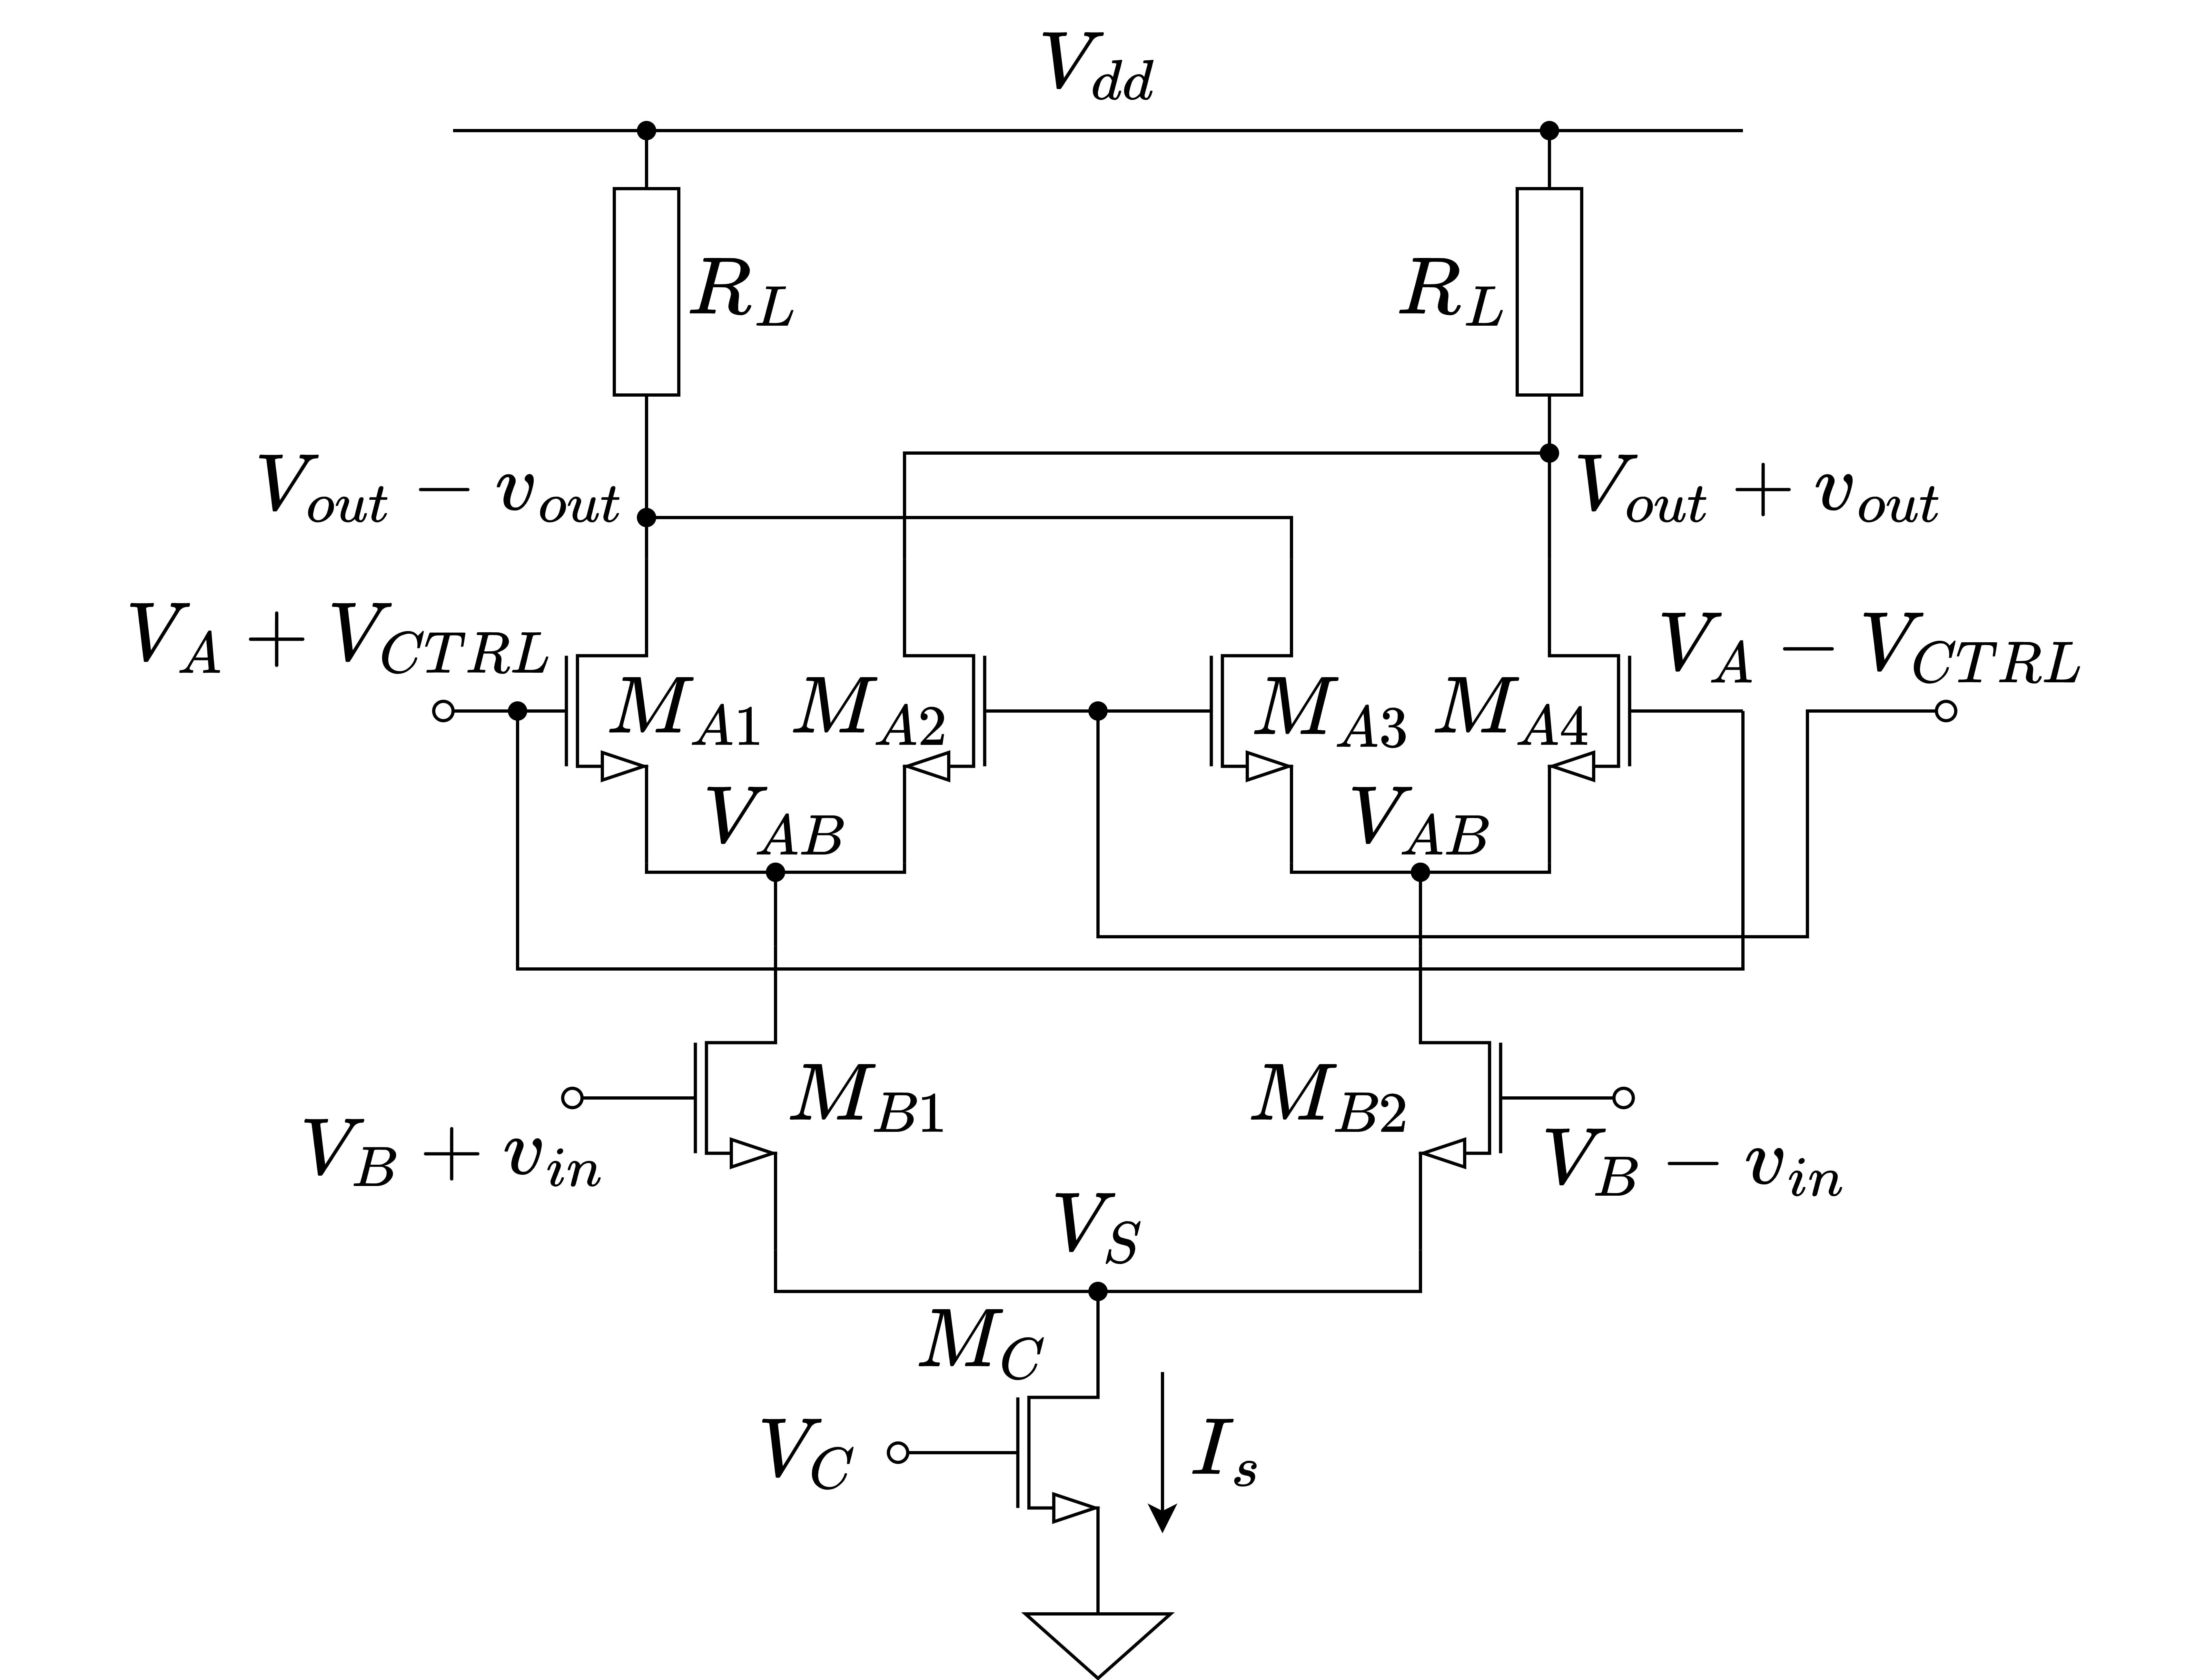
\includegraphics[width=160mm]{figures/chapter2/gilbert.png}
                \caption{ギルバート乗算回路}
                \label{fig:2_gilbert}
            \end{center}
        \end{figure}
        ギルバート乗算回路は$v_{in}$と$V_{CTRL}$に差動で信号を入力することで二つの入力信号に比例した電圧出力を差動で出力することができる。ここで、$M_{B}$の差動対は入力信号に比例した電流を$M_{A}$のソースから引き込む。さらに$M_{A}$の動作点が制御電圧$V_{CTRL}$に比例して変動することに注意すると負荷抵抗に流れる電流が二つの入力に比例していることが分かる。詳細は次節にて導出する。


    \section{小信号解析}
        \subsection{動作点の変動}   \label{ch:gilbert_valiable_gm}
            小信号解析を行うにあたり$M_{A}$の扱いが問題となる。小信号解析ではMOSFETの出力が線形に近似できるような小信号入力に対して行うが、動作点が変動すると線形な近似が合わなくなる。この問題を扱うために、まず図\ref{fig:2_OP}に示す差動ゲート接地の差動対について考える。\par
            \begin{figure}[b]
                \begin{center}
                    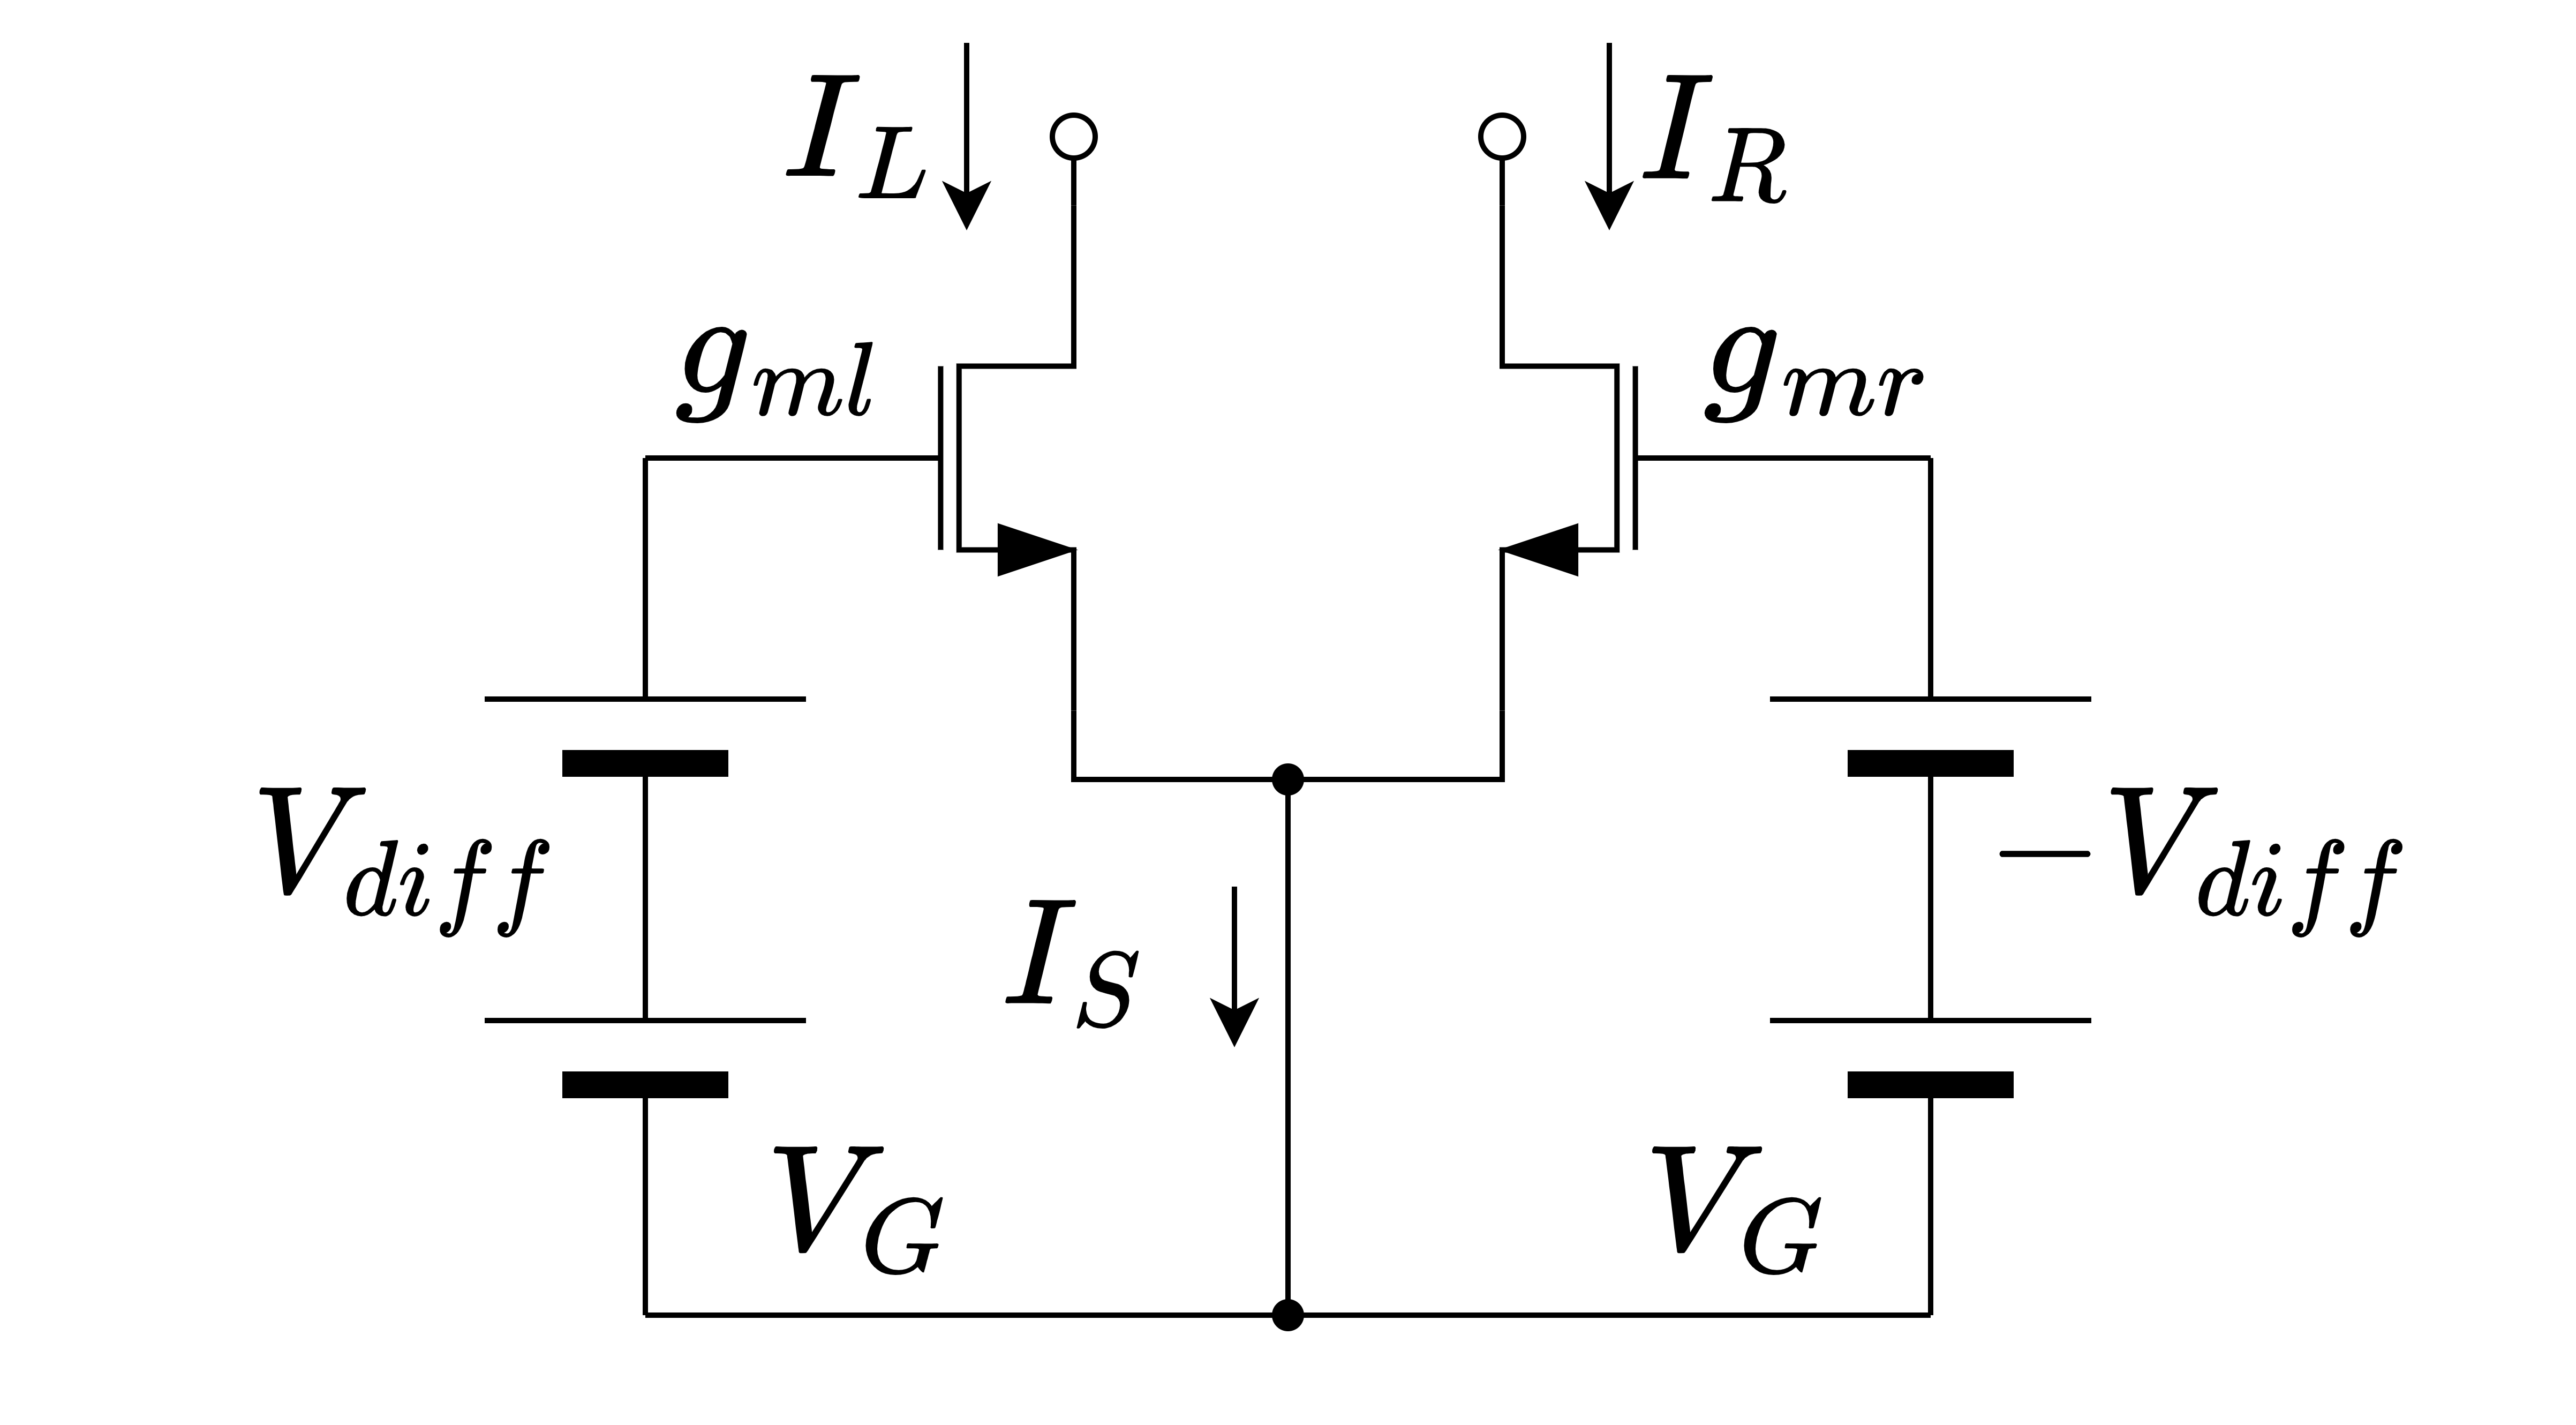
\includegraphics[width=80mm]{figures/chapter2/OperatingPoint.png}
                    \caption{ゲート接地の差動対}
                    \label{fig:2_OP}
                \end{center}
            \end{figure}
            一般に、MOSFETのドレイン電流は二乗則に従い、ゲートソース間電圧$V_{GS}$、しきい電圧$V_{th}$と形状などによって決まる固有の係数$K$を用いて
            \begin{align}
                I_{D}=K(V_{GS}-V_{th})^{2}  \label{eq:2_id}
            \end{align}
            と表せる。さらに、MOSFETのトランスコンダクタンスはドレイン電流をゲートソース間電圧で偏微分したものであるので差動成分が$0$、つまり$V_{diff}=0$のときトランスコンダクタンスを$g_{m}$とすると式(\ref{eq:2_id})を用いて
            \begin{align}
                g_{m}&=\frac{ \partial I_{D} }{ \partial V_{GS} }   \notag\\
                &=2K(V_{GS}-V_{th})     \label{eq:2_gm}
            \end{align}
            となる。次に差動成分$V_{diff}\neq0$のとき、左右のMOSFETのトランスコンダクタンスは
            \begin{align}
                g_{ml}&=2K\left\{ (V_{G}+V_{diff}) -V_{th} \right\}     \notag\\
                &=g_{m}+2KV_{diff}      \notag\\
                g_{mr}&=2K\left\{ (V_{G}-V_{diff}) -V_{th} \right\}     \notag\\
                &=g_{m}-2KV_{diff}      \notag
            \end{align}
            と計算できるので、$2KV_{diff}\equiv\Delta g_{m}$とおけば
            \begin{align}
                g_{ml}&=g_{m}+\Delta g_{m}   \label{eq:2_dgml}\\
                g_{mr}&=g_{m}-\Delta g_{m}   \label{eq:2_dgmr}
            \end{align}
            と求められた。したがって、ゲート接地増幅回路ではゲート電圧に比例したトランスコンダクタンスを得ることができる。
            \newpage
            
        \subsection{小信号等価回路}
            次に小信号等価回路を考えるが、ここでギルバート乗算回路は差動対の組み合わせでできているため、半回路を考えることで回路全体の小信号解析を行うことができる。
            \begin{figure}[b]
                \begin{center}

                    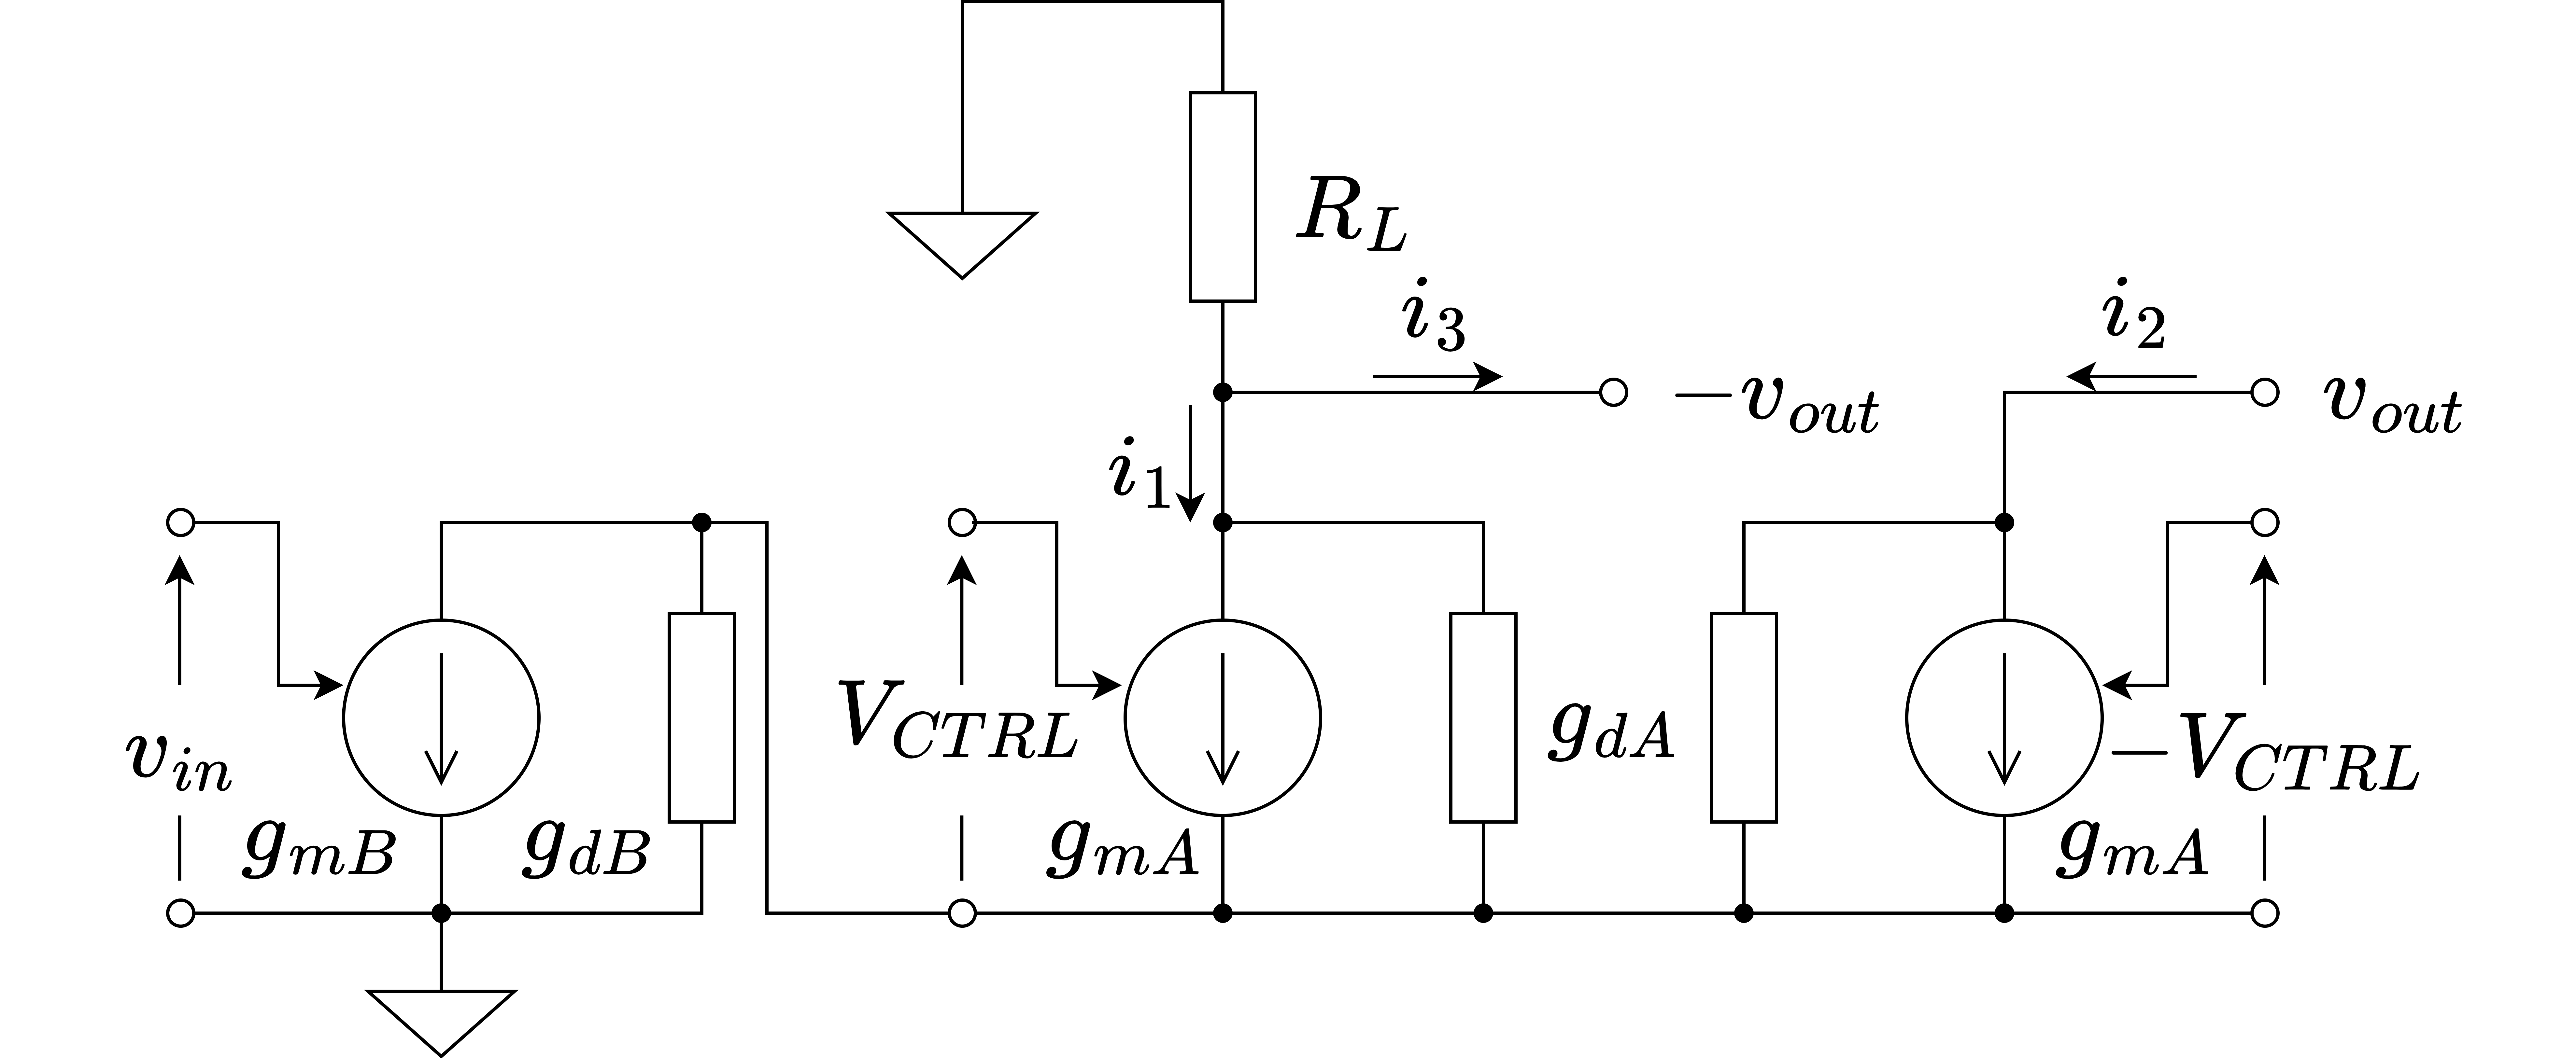
\includegraphics[width=125mm]{figures/chapter2/halfeq.png}
                    \caption{ギルバート乗算回路の小信号半回路}
                    \label{fig:2_half}

                \end{center}

            \end{figure}
            そこで図\ref{fig:2_gilbert}の$M_{A1},M_{A2},M_{B1}$についての半回路は$V_{S}$が交流的に接地されていることに留意すると、図\ref{fig:2_half}に示すようになる。この時、接点$AB$にKCLを用いると
            \begin{align}
                g_{mB}v_{in}+g_{dB}v_{AB}&=(g_{m}+\Delta g_{m})(-v_{AB})+g_{dA}(v_{outm}-v_{AB})    \notag\\
                &\quad\quad\quad\quad +(g_{m}-\Delta g_{m})(-v_{AB})+g_{dA}(v_{outp}-v_{AB})     \notag\\
                v_{AB}&=-\frac{g_{mB}}{2g_{m}+2g_{dA}+g_{dB}}v_{in}     \label{eq:2_vab}
            \end{align}
            と書ける。さらに、完全差動回路であることを踏まえると$i_{3}=-i_{2}$、$v_{outp}=-v_{outm}$という関係が成り立つ。また最終的な出力電圧を$v_{out}:=v_{outp}-v_{outm}$と定義する。これに留意して負荷抵抗$R_{L}$に流れる電流$i_{outm}$は
            \begin{align}
                i_{outm}&=i_{1}+i_{2}       \notag\\
                &=(g_{m}+\Delta g_{m})(-v_{AB})+g_{dA}(v_{outm}-v_{AB})       \notag\\
                &\quad\quad\quad\quad -\left\{  (g_{m}-\Delta g_{m})(-v_{AB})+g_{dA}(v_{outp}-v_{AB})  \right\}   \notag\\
                &=-2(\Delta g_{m}v_{AB}+g_{dA}v_{out})      \label{eq:2_iout}
            \end{align}
            と表せる。オームの法則を用いると
            \begin{align}
                v_{out}&=\left\{ \left(0-R_{L}i_{outp}\right) - \left(0-R_{L}i_{outm}\right) \right\}    \notag\\
                &=\frac{ 4R_{L} }{1+2R_{L}g_{dA}}\Delta g_{m}v_{AB}     \notag
            \end{align}
            と計算できる。ここで、$g_{m}>>g_{dA},g_{dB}$を仮定し\ref{ch:gilbert_valiable_gm}の結果と式(\ref{eq:2_vab})を用いると出力電圧は
            \begin{align}
                v_{out}=\frac{ 8KR_{L} }{ 1+2R_{L} }\cdot\frac{ g_{mB} }{ 2g_{m} }\cdot V_{CTRL}\cdot v_{in}       \label{eq:2_vout}
            \end{align}
            と表すことができる。ここで、$V_{CTRL}$と$K$はそれぞれ$M_{A}$に与える制御電圧とトランスコンダクタンス係数である。以上より、小信号を入力した際には出力として入力電圧$v_{in}$と制御電圧$V_{CTRL}$に比例した電圧を得る、すなわち乗算ができることが確かめられた。
            \newpage


    \section{出力範囲}
        次にギルバート乗算回路の出力範囲を考える。適切に乗算が行える条件はMOSFETが遮断領域に入らないことであるとすると、制約条件として各MOSFETにおいて
        \begin{subequations}
        \begin{empheq}[left={\empheqlbrace}]{align}
            &V_{GS}-V_{th}<V_{DS}          \\
            &V_{th}<V_{GS}              
        \end{empheq}        \label{eq:2_binding_conditions}
        \end{subequations}
        を満たす必要がある。ただし、$V_{GS}$、$V_{DS}$、$V_{th}$はゲートソース間電圧、ドレインソース間電圧、しきい電圧である。これを図\ref{fig:2_gilbert}の各MOSFETに用いると
        \begin{empheq}[left={M_{A}:\empheqlbrace}]{align}
            &V_{A}+V_{CTRL}-V_{AB}-V_{th}<V_{out}-v_{out}-V_{AB}        \tag{\ref{eq:2_ma_binding_pre}.a}   \\
            &V_{th}<V_{A}-V_{CTRL}-V_{AB}                               \tag{\ref{eq:2_ma_binding_pre}.b}
        \end{empheq}        \label{eq:2_ma_binding_pre}
        \begin{empheq}[left={M_{B}:\empheqlbrace}]{align}
            &V_{B}+v_{in}-V_{S}-V_{th}<V_{AB}-V_{S}     \tag{\ref{eq:2_mb_binding_pre}.a} \\
            &V_{th}<V_{B}-v_{in}-V_{S}                  \tag{\ref{eq:2_mb_binding_pre}.b}
        \end{empheq}        \label{eq:2_mb_binding_pre}
        \begin{empheq}[left={M_{C}:\empheqlbrace}]{align}
            &V_{C}-V_{th}<V_{S}     \tag{\ref{eq:2_mc_binding_pre}.a} \\
            &V_{th}<V_{C}           \tag{\ref{eq:2_mc_binding_pre}.b}
        \end{empheq}        \label{eq:2_mc_binding_pre}
        と表現することができる。$M_{A},M_{B}$の.a不等式には両辺にソース電位が含まれているのでそれを消去すると
        \begin{empheq}[left={M_{A}:\empheqlbrace}]{align}
            &V_{A}+V_{CTRL}-V_{th}<V_{out}-v_{out}        \tag{\ref{eq:2_ma_binding}.a'}   \\
            &V_{th}<V_{A}-V_{CTRL}-V_{AB}                 \tag{\ref{eq:2_ma_binding}.b'}
        \end{empheq}        \label{eq:2_ma_binding}
        \begin{empheq}[left={M_{B}:\empheqlbrace}]{align}
            &V_{B}+v_{in}-V_{th}<V_{AB}     \tag{\ref{eq:2_mb_binding}.a'} \\
            &V_{th}<V_{B}-v_{in}-V_{S}      \tag{\ref{eq:2_mb_binding}.b'}
        \end{empheq}        \label{eq:2_mb_binding}
        とまとめられる。



%    \begin{figure}
%        \begin{center}
%            \includegraphics[width=125mm]{figures/chapter2}
%            \caption{}
%            \label{fig:2_}
%        \end{center}
%    \end{figure}

%    \begin{empheq}[left={\empheqlbrace}]{align}
%    \end{empheq}        \label{eq:}

%\chapter{カレントミラーを組み合わせた折り返し型アナログ乗算回路}

    \section{回路構成}
        序論で述べたS/N比向上のための方針として、折り返しカスコードの構成をとることが考えられる。図\ref{fig:3_folded_gilbert}に折り返しカスコード型の乗算回路を示す。
        \begin{figure}[!b]
            \begin{center}
                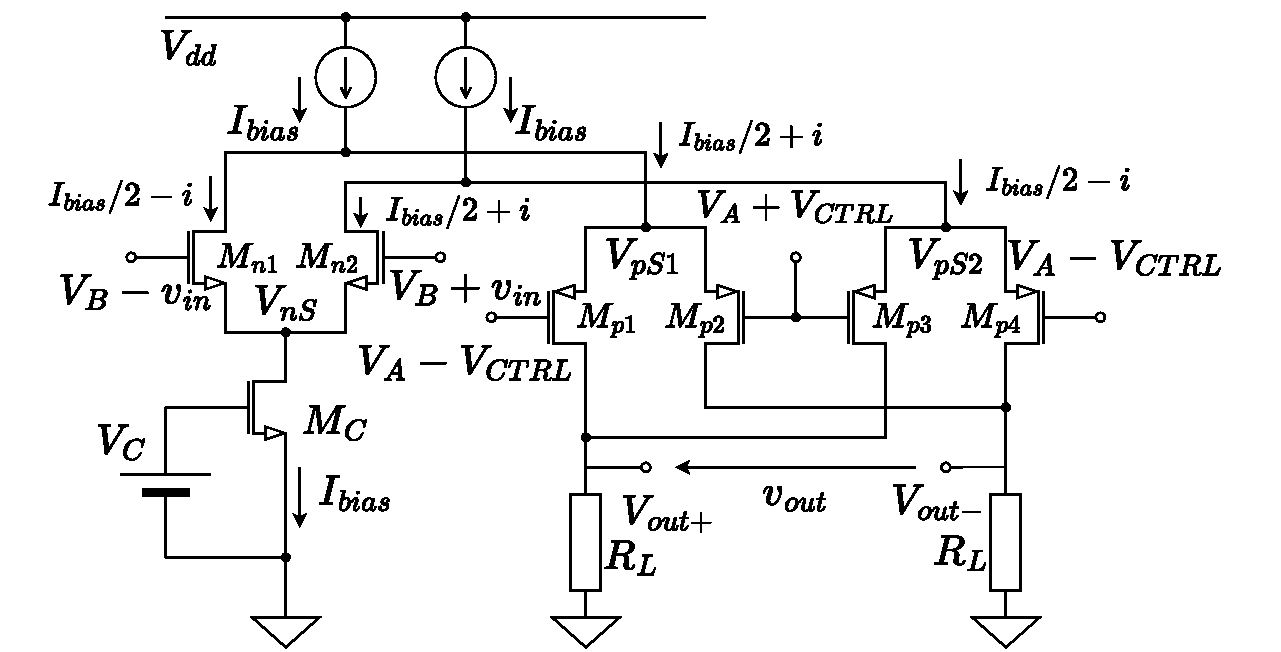
\includegraphics[width=0.99\linewidth]{figures/chapter3/folded_gilbert.pdf}
                \caption{折り返しカスコード型乗算回路}
                \label{fig:3_folded_gilbert}
            \end{center}
        \end{figure}
        この構造では定電流源を用いることで各$\mathrm{M_{B}}$に流れる信号電流の増減が$\mathrm{M_{p}}$に反転して伝えられる。ゲート接地増幅回路としてはpMOSFET($\mathrm{M_{p1}}$~$\mathrm{M_{p4}}$)を用いることで制御電圧に比例したトランスコンダクタンスを得る。このような折り返しカスコード型の構造をとることで出力電圧は$M_{p}$と電流源のpMOSFETで分圧するため、入力電圧分出力振幅が広がることが予測される。しかし左右それぞれにバイアス電流を流すため消費電流が増加する。さらにpMOSFETを小信号に使用するためどうしてもnMOSFETのみのギルバート乗算回路よりも遮断周波数が低下するといったデメリットが考えられる。$\mathrm{RHOM\;0.18\mu\;m\;Process}$にてギルバート乗算回路と折り返しカスコード型の乗算回路をバイアス電流が同じになるように設計したときのそれぞれの素子値を表\ref{table:3_gilbert_param}、表\ref{table:3_folded_gilbert_param}に示す。またこの素子値におけるシミュレーションでの周波数特性を図\ref{fig:3_gilbert_ac}、図\ref{fig:3_folded_gilbert_ac}にそれぞれ示す。
        \begin{table}[!b]
            \begin{minipage}[t]{.45\textwidth}
                \begin{center}
                    \caption{比較用に設計したギルバート乗算回路}
                    \label{table:3_gilbert_param}
                    \begin{tabular}{c|c|r}
                        \hline
                        \multicolumn{2}{c}{Gilbert}   & \multicolumn{1}{c}{Value}     \\
                        \hline\hline
                        &   Channel Length   &   0.72 $\mathrm{\mu m}$   \\
                        \cline{2-3}
                        $\mathrm{M_{A}}$   &   Channel Width   &   4.27 $\mathrm{\mu m}$   \\
                        \cline{2-3}
                            &   Multifinger   & 10    \\
                        \hline
                        &   Channel Length   &   0.72 $\mathrm{\mu m}$   \\
                        \cline{2-3}
                        $\mathrm{M_{B}}$   &   Channel Width   &   4.27 $\mathrm{\mu m}$   \\
                        \cline{2-3}
                            &   Multifinger   & 20    \\
                        \hline
                        &   Channel Length   &   0.72 $\mathrm{\mu m}$   \\
                        \cline{2-3}
                        $\mathrm{M_{C}}$   &   Channel Width   &   11.6 $\mathrm{\mu m}$   \\
                        \cline{2-3}
                            &   Multifinger   & 40    \\
                        \hline
                        \multicolumn{2}{c|}{$\mathrm{V_{dd}}$} &   1.8 $\mathrm{V}$   \\
                        \hline
                        \multicolumn{2}{c|}{$\mathrm{V_{A}}$} &   1.59 $\mathrm{V}$   \\
                        \hline
                        \multicolumn{2}{c|}{$\mathrm{V_{B}}$} &   1.09 $\mathrm{V}$   \\
                        \hline
                        \multicolumn{2}{c|}{$\mathrm{V_{C}}$} &   0.65 $\mathrm{V}$   \\
                        \hline
                        \multicolumn{2}{c|}{$\mathrm{R_{L}}$} &   300 $\mathrm{\Omega}$   \\
                        \hline
                    \end{tabular}
                \end{center}                
            \end{minipage}
            %
            \hfill
            %
            \begin{minipage}[t]{.45\textwidth}
                \begin{center}
                    \caption{設計した折り返しカスコード型乗算回路}
                    \label{table:3_folded_gilbert_param}
                    \begin{tabular}{c|c|r}
                            \hline
                            \multicolumn{2}{c}{Folded Cascode}   & \multicolumn{1}{c}{Value}     \\
                            \hline\hline
                            &   Channel Length   &   0.72 $\mathrm{\mu m}$   \\
                            \cline{2-3}
                            $\mathrm{M_{p}}$   &   Channel Width   &   20 $\mathrm{\mu m}$   \\
                            \cline{2-3}
                                &   Multifinger   & 10    \\
                            \hline
                            &   Channel Length   &   0.72 $\mathrm{\mu m}$   \\
                            \cline{2-3}
                            $\mathrm{M_{B}}$   &   Channel Width   &   4.27 $\mathrm{\mu m}$   \\
                            \cline{2-3}
                                &   Multifinger   & 20    \\
                            \hline
                            &   Channel Length   &   0.72 $\mathrm{\mu m}$   \\
                            \cline{2-3}
                            $\mathrm{M_{C}}$   &   Channel Width   &   11.6 $\mathrm{\mu m}$   \\
                            \cline{2-3}
                                &   Multifinger   & 40    \\
                            \hline
                            \multicolumn{2}{c|}{$\mathrm{V_{dd}}$} &   1.8 $\mathrm{V}$   \\
                            \hline
                            \multicolumn{2}{c|}{$\mathrm{V_{A}}$} &   1.59 $\mathrm{V}$   \\
                            \hline
                            \multicolumn{2}{c|}{$\mathrm{V_{B}}$} &   1.09 $\mathrm{V}$   \\
                            \hline
                            \multicolumn{2}{c|}{$\mathrm{V_{C}}$} &   0.65 $\mathrm{V}$   \\
                            \hline
                            \multicolumn{2}{c|}{$\mathrm{R_{L}}$} &   300 $\mathrm{\Omega}$   \\
                            \hline
                    \end{tabular}
                \end{center}
            \end{minipage}
        \end{table}
        \begin{figure}[!b]
            \centering
            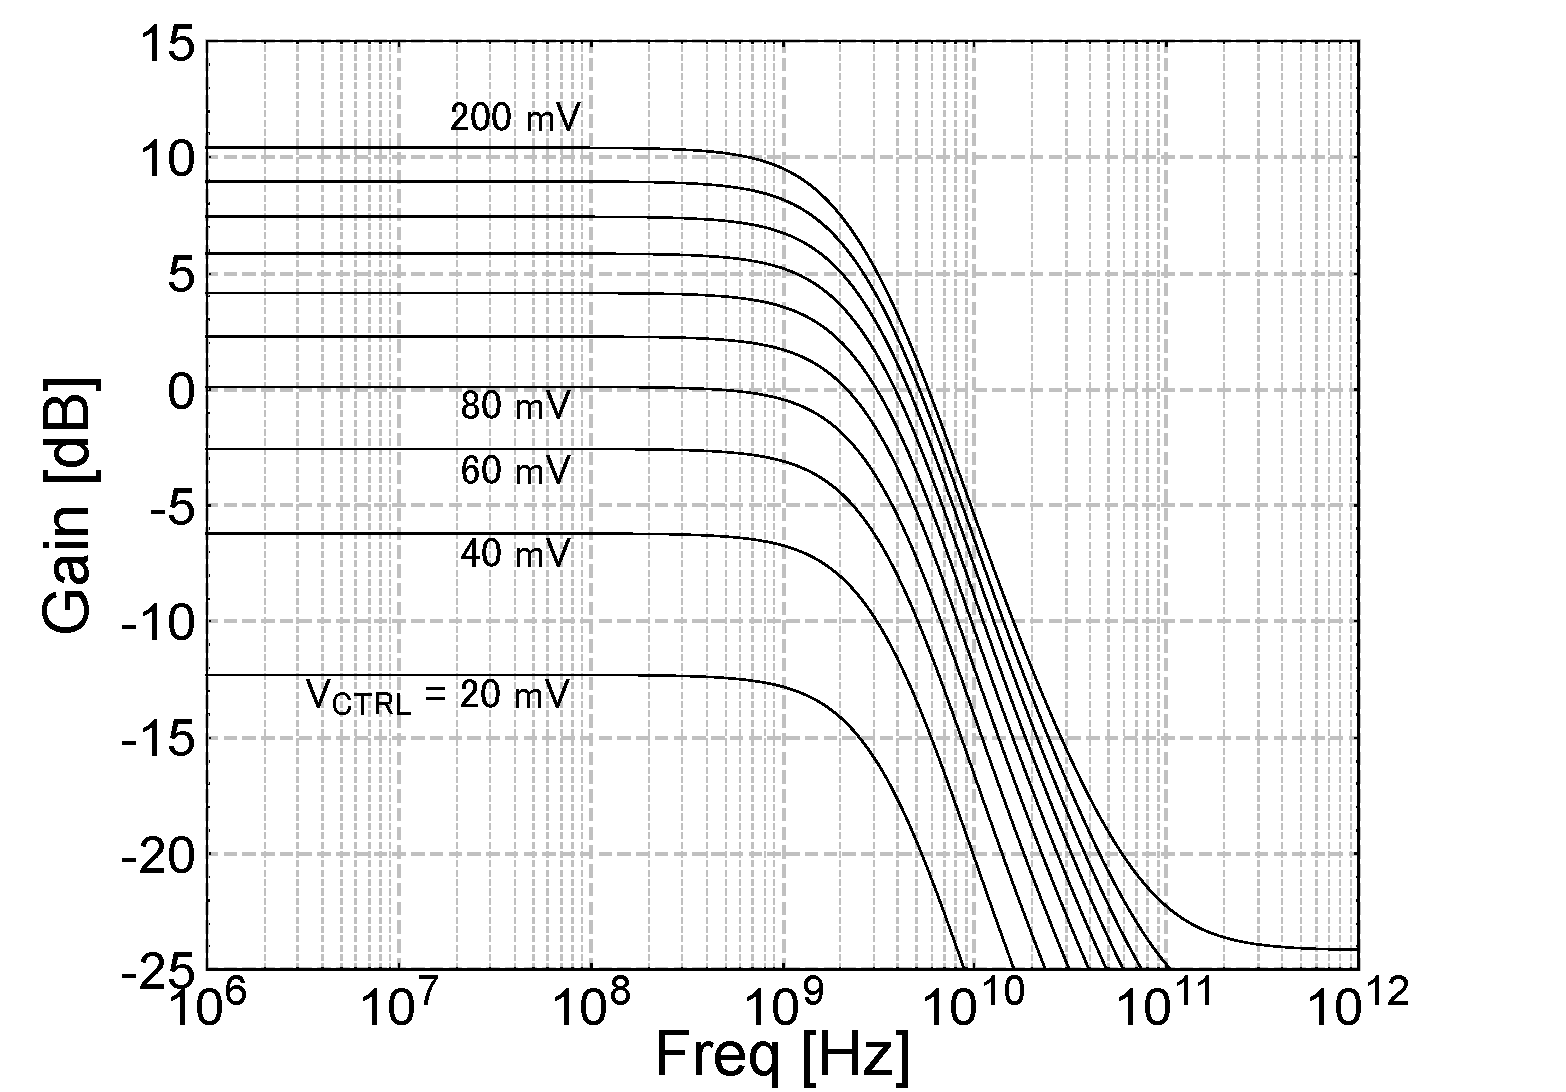
\includegraphics[width=0.99\textwidth]{figures/chapter3/previous_ac.pdf}
            \caption{ギルバート乗算回路の周波数特性}
            \label{fig:3_gilbert_ac}
        \end{figure}
        \begin{figure}[!b]
            \centering
            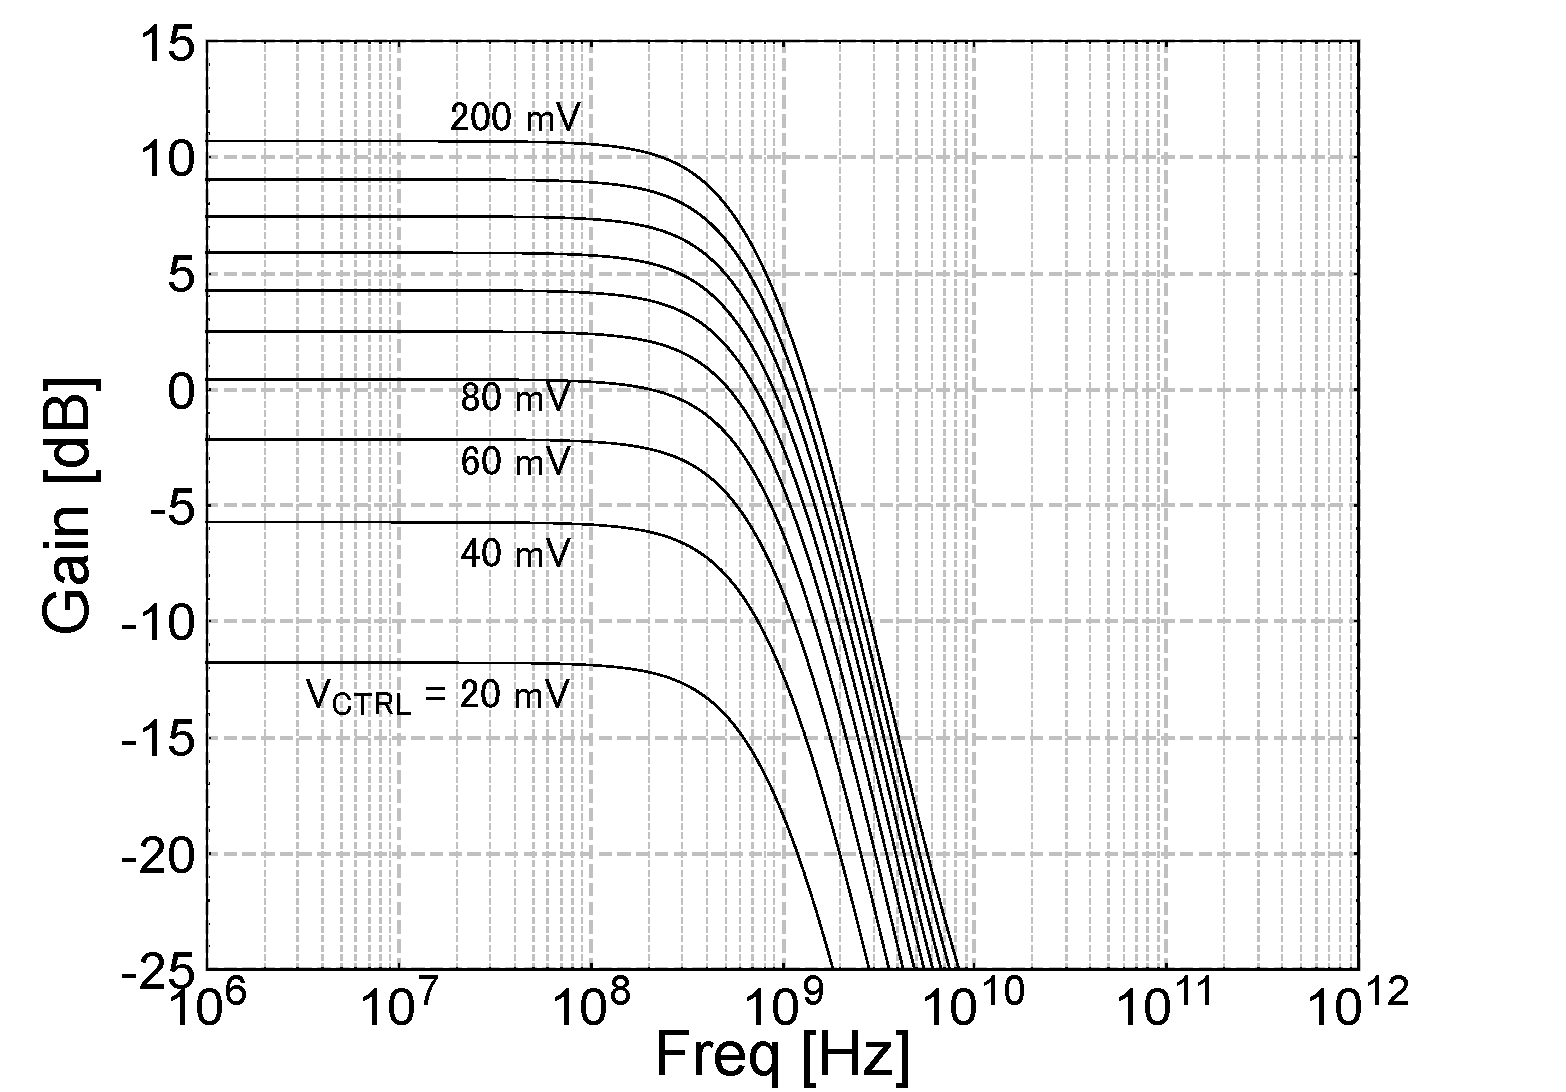
\includegraphics[width=0.99\textwidth]{figures/chapter3/folded_ac.pdf}
            \caption{折り返しカスコード型の周波数特性}
            \label{fig:3_folded_gilbert_ac}
        \end{figure}
        \clearpage
        今回の設計ではトランスコンダクタンスも揃っているので利得は同程度であるが、遮断周波数は1桁程度落ちてしまっている。本論文での目的はS/N比を向上させるために出力範囲を拡大することであるが、フォトニックリザバに用いることを想定すると周波数特性が構造的にギルバート乗算回路よりも悪化するのは避けたい。そこでpMOSFETを使用せずに信号の折り返しを行うことで出力範囲を拡大できるのではないかと考え、これを実現する回路を図\ref{fig:3_folded_mirror_gilbert}に示し、これをカレントミラーを組み合わせた折り返し型乗算回路とした。\par
        \begin{figure}[!b]
            \begin{center}
                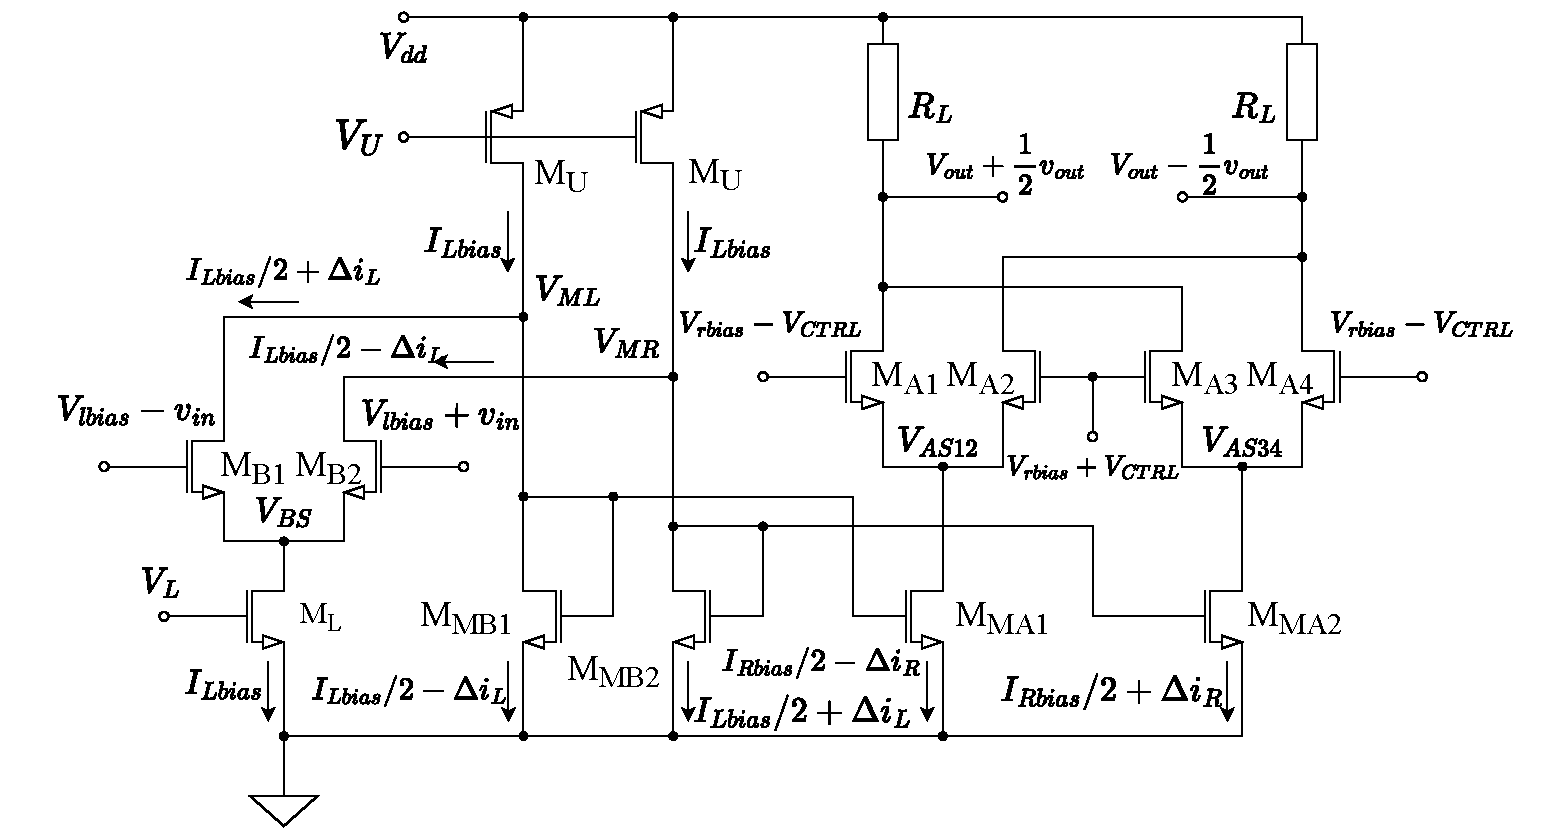
\includegraphics[width=0.99\textwidth]{figures/chapter3/NtoNFolded.pdf}
                \caption{カレントミラーを組み合わせた折り返し型乗算回路}
                \label{fig:3_folded_mirror_gilbert}
            \end{center}
        \end{figure}
        $\mathrm{M_{U},M_{L}}$はともに電流源として用いており、定電流$I_{Lbias}$を入力のMOSFETである$\mathrm{M_{B}}$とカレントミラーの参照電流を流す$M_{MB}$で分流する。これにより、入力の差動対によって$v_{in}$に比例した信号電流を符号を逆転させ$M_{MB}$に流す。カレントミラーのコピー側である$\mathrm{M_{MA}}$には$\mathrm{M_{MB}}$と$\mathrm{M_{MA}}$の形状比と$v_{in}$に比例した電流を流すことができる。これにより制御電圧を印加する$\mathrm{M_{A}}$に流れるバイアス電流を変動させる。$\mathrm{M_{A}}$はゲート接地増幅回路であり、\ref{ch:gilbert_valiable_gm}節での議論からトランスコンダクタンスは$V_{CTRL}$に比例しており、負荷抵抗に流れる電流を$V_{in}$と$V_{CTRL}$に比例したものにすることができる。そして負荷抵抗によって電流を電圧に変換する。このようにしてカレントミラーと差動対で電流を分流することで折り返しカスコード型の様に信号を伝達することができるのではないかと予測し、図\ref{fig:3_folded_mirror_gilbert}の構成を考えた。

    \section{小信号解析}
        前節では今回提案する構成によって乗算ができると考える理由を述べたが、本節では小信号解析により提案回路を用いたアナログ乗算が可能であることを示す。\par
        図\ref{fig:3_folded_mirror_gilbert}はギルバート乗算回路同様差動回路であるため差動半回路を考えることで回路全体の小信号解析を行うことができる。したがって半回路として考える部分を図\ref{fig:3_folded_mirror_gilbert_half}に示す。また、この時の小信号等価半回路を図\ref{fig:3_folded_mirror_half}に示す。
        \begin{figure}[!b]
            \centering
            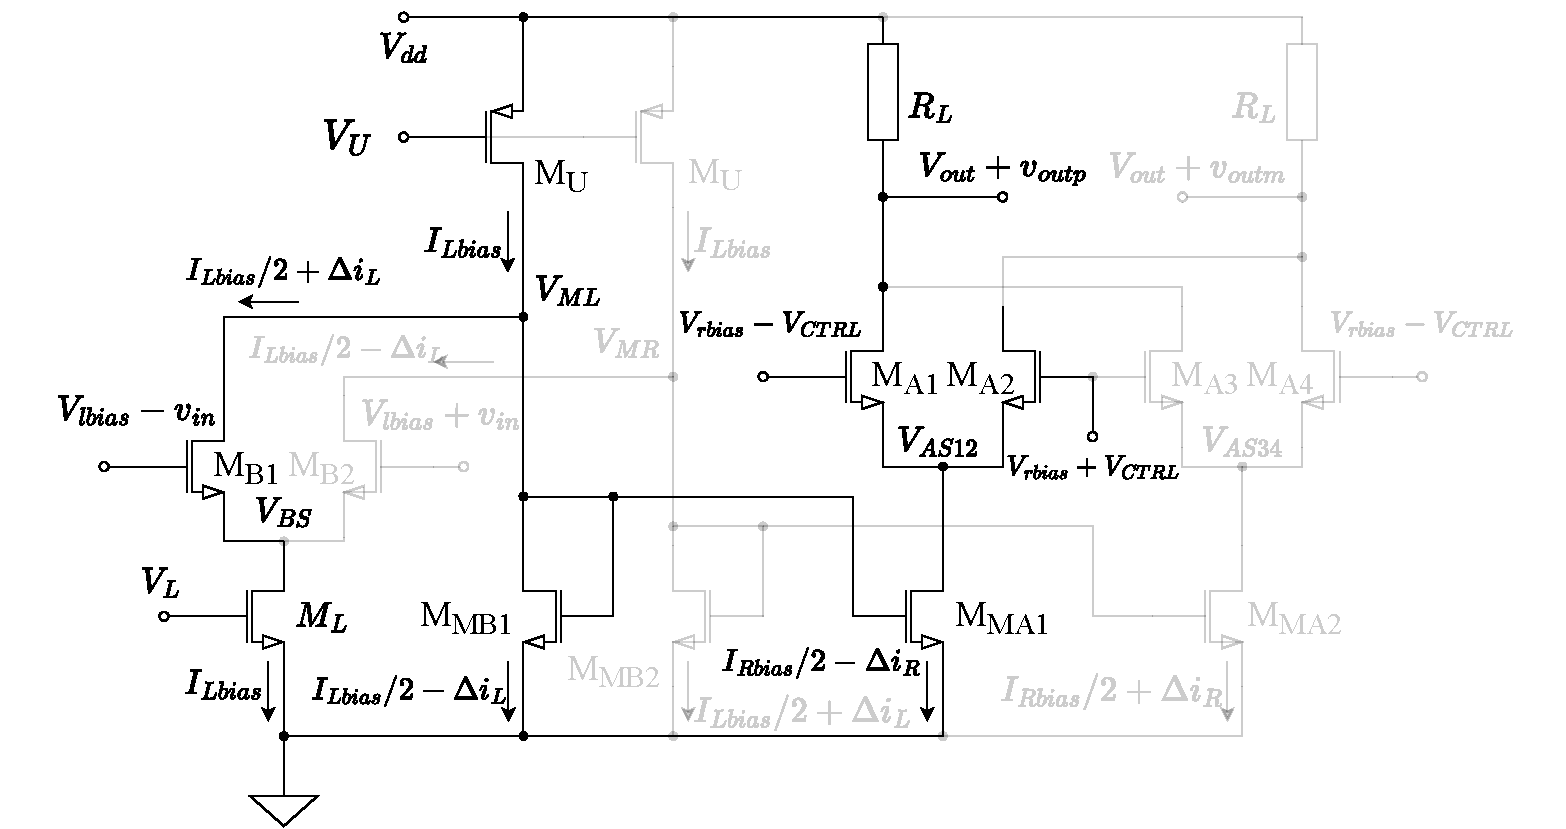
\includegraphics[width=0.99\textwidth]{figures/chapter3/NtoNFolded_half.pdf}
            \caption{カレントミラーを組み合わせた折り返し型アナログ乗算回路の半回路として考える部分}
            \label{fig:3_folded_mirror_gilbert_half}
        \end{figure}
        \begin{figure}[!b]
            \centering
            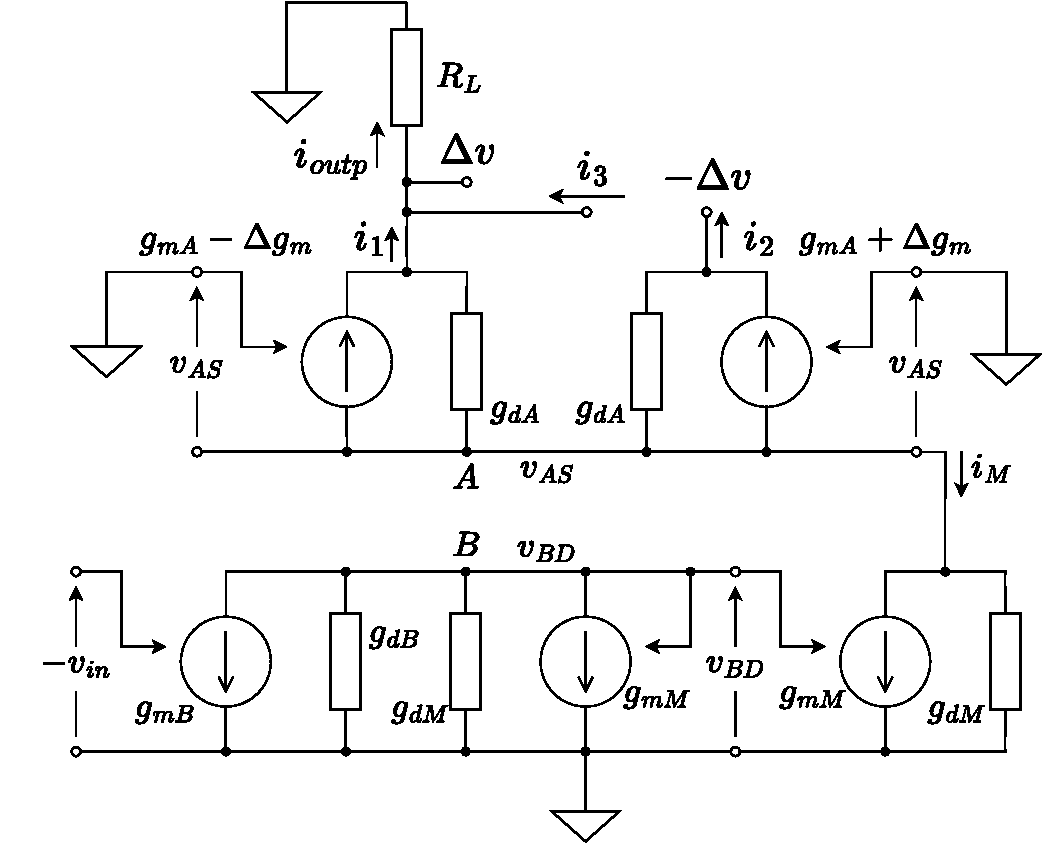
\includegraphics[width=0.99\textwidth]{figures/chapter3/NtoNHalfDiffEqual.pdf}
            \caption{カレントミラーを組み合わせた折り返し型アナログ乗算回路の小信号半回路}
            \label{fig:3_folded_mirror_half}
        \end{figure}
        \clearpage
        ここで$g_{mB},g_{mMB},g_{mMA},g_{mA}$はそれぞれ$\mathrm{M_{B},M_{MB},M_{MA},M_{A}}$のトランスコンダクタンスであり、$g_{dB},g_{dMB},g_{dMA},g_{dA}$は$\mathrm{M_{B},M_{MB},M_{MA},M_{A}}$のドレインソース間抵抗である。また$R_{L}$は負荷抵抗であり、$v_{AS},v_{BD}$はそれぞれ接点A,Bの電位とする。この時、接点BにKCLを用いると$v_{BD}$は
        \begin{align}
            0&=g_{mB}(-v_{in})+(g_{dB}+g_{dMB})v_{BD}+g_{mMB}v_{BD}     \notag\\
            v_{BD}&=\frac{g_{mB}}{ g_{mMB}+g_{dMA}+g_{dMB} }v_{in}      \notag
        \end{align}
        と表せる。ここで、$g_{mB}>>g_{dMA},g_{dMB}$を仮定すると
        \begin{align}
            v_{BD}\approx \frac{g_{mB}}{g_{mMB}}v_{in}      \label{eq:3_vbd}
        \end{align}
        と近似することができる。次に$i_{A1},i_{A2}$はそれぞれ
        \begin{align}
            i_{A1}&=(g_{mA}-\Delta g_{m})(-v_{AS})+g_{dA}(v_{outp}-v_{AS})      \label{eq:3_ia1}\\
            i_{A2}&=(g_{mA}+\Delta g_{m})(-v_{AS})+g_{dA}(v_{outm}-v_{AS})      \label{eq:3_ia2}   
        \end{align}
        であることを用いると、接点AについてのKCLを考えることで$v_{AS}$は
        \begin{align*}
            g_{mMA}v_{BD}+g_{dMA}v_{AS}&=i_{A1}+i_{A2}   \\
            &=(g_{mA}-\Delta g_{m})(-v_{AS})+g_{dA}(v_{outp}-v_{AS})    \\
            &\quad\quad\quad\quad +(g_{mA}+\Delta g_{m})(-v_{AS})+g_{dA}(v_{outm}-v_{AS})       \\
            &=-2g_{mA}v_{AS}-2g_{dA}v_{AS}  \\
            v_{AS} &= -\frac{ g_{mMA} }{ 2g_{mA}+2g_{dA}+g_{dMA} }v_{BD}
        \end{align*}
        と計算できる。さらに$g_{mMA}>>2g_{dA},g_{dMA}$を仮定すると
        \begin{align}
            V_{AS} \approx -\frac{g_{mMA}}{2g_{mA}} v_{BD}      \label{eq:3_vas}
        \end{align}
        の近似ができる。ここで図\ref{fig:3_folded_mirror_half}が差動回路であることに注意すると、\mbox{$i_{A3}=-i_{A2}$} \mbox{$v_{outp}=-v_{outm}$}の関係が成り立つので
        \begin{align}
            i_{outp}&=i_{A1}+i_{A3}     \notag\\
            &=i_{A1}-i_{A2}     \notag\\
            &=2\Delta g_{m}v_{AS}+2g_{dA}v_{outp}     \label{eq:3_ioutp}
        \end{align}
        と$v_{outp}$を用いて$i_{outp}$を表すことができた。接点OについてのKVLを考えると
        \begin{align}
            v_{outp}&=0-R_{L}i_{outp}       \notag\\
            &=-R_{L}\left( 2\Delta g_{m}v_{AS}+2g_{dA}v_{outp}  \right)       \notag\\
            &=-\frac{ 2R_{L} }{ 1+2R_{L}g_{dA} } \cdot \Delta g_{m}v_{AS}       \label{eq:3_voutp}    
        \end{align}
        であるので、出力電圧$v_{out}$を$v_{out}:=v_{outp}-v_{outm}$とすれば$v_{outp}=-v_{outm}$であることに留意すると
        \begin{align*}
            v_{out}&=2v_{outp}  \\
            &=-\frac{ 4R_{L} }{ 1+2R_{L}g_{dA} } \cdot \Delta g_{m}v_{AS}
        \end{align*}
        と計算できる。ここで式(\ref{eq:3_vbd})、(\ref{eq:3_vas})を代入すると
        \begin{align*}
            v_{out}=\frac{ g_{mB} }{ g_{mA} }\cdot\frac{ g_{mMA} }{ g_{mMB} }\cdot\frac{ 2R_{L} }{ 1+2R_{L} g_{dA}}\cdot\Delta g_{m}v_{in}
        \end{align*}
        である。さらに\ref{ch:gilbert_valiable_gm}の結論を用いれば、$\mathrm{M_{A}}$のトランスコンダクタンス係数を$K$としたとき$\Delta g_{m}=2KV_{CTRL}$なので
        \begin{align}
            v_{out}=\frac{ g_{mB} }{ g_{mA} }\cdot\frac{ g_{mMA} }{ g_{mMB} }\cdot\frac{ 4KR_{L} }{ 1+2R_{L} g_{dA}}\cdot V_{CTRL}\cdot v_{in}      \label{eq:3_vout}
        \end{align}
        と計算することができた。したがってカレントミラーを組み合わせた折り返し型乗算回路は入力電圧$v_{in}$と制御電圧$V_{CTRL}$に比例した出力を得ることができる。特にカレントミラーの形状比が同一である場合、$g_{mMA}=g_{mMB}$となるため、ギルバート乗算回路の出力と一致することが分かる。


    \section{出力範囲}
        次に、\ref{ch:2_range}と同様の方法で出力範囲を求めギルバート乗算回路と比較を行う。まず、適切に動作する条件をすべてのMOSFETが飽和領域で動作することするための式(\ref{eq:2_binding_conditions})を再掲すると
        \begin{subequations}
            \begin{empheq}[left={\empheqlbrace}]{align*}
                &V_{GS}-V_{th}<V_{DS}          \\
                &V_{th}<V_{GS}              
            \end{empheq}
        \end{subequations}
        であった。これを図\ref{fig:3_folded_mirror_gilbert}の各MOSFETに適用すると
        \begin{subequations}
            \begin{empheq}[left={M_{A}:\empheqlbrace}]{align}
                &V_{rbias}+V_{CTRL}-V_{AS}-V_{th}<V_{out-\frac{1}{2}}-V_{AS}        \\
                &V_{th}<V_{rbias}-V_{CTRL}-V_{AS}
            \end{empheq}        \label{eq:3_ma_binding}
        \end{subequations}
        \begin{subequations}
            \begin{empheq}[left={M_{MA}:\empheqlbrace}]{align}
                &V_{M}-V_{th}<V_{AS}        \\
                &V_{th}<V_{dd}-V_{U}
            \end{empheq}        \label{eq:3_mma_binding}
        \end{subequations}
        \begin{subequations}
            \begin{empheq}[left={M_{U}:\empheqlbrace}]{align}
                &V_{dd}+v_{in}-V_{BS}-V_{th}<V_{dd}-V_{BS}      \\
                &V_{th}<V_{dd}-V_{U}
            \end{empheq}        \label{eq:3_mu_binding}
        \end{subequations}
        \begin{subequations}
            \begin{empheq}[left={M_{B}:\empheqlbrace}]{align}
                &V_{lbias}+v_{in}-V_{BS}-V_{th}<V_{M}-V_{BS}        \\
                &V_{th}<V_{lbias}-v_{in}-V_{BS}
            \end{empheq}        \label{eq:3_mb_binding}
        \end{subequations}
        \begin{subequations}
            \begin{empheq}[left={M_{L}:s\empheqlbrace}]{align}
                &V_{L}-V_{th}<V_{BS}        \\
                &V_{th}<V_{L}
            \end{empheq}        \label{eq:3_ml_binding}
        \end{subequations}
        という5つの不等式が得られる。ただし、$\mathrm{M_{MA}}$に関してはダイオード接続になっているので常に飽和領域で動作する。まず$\mathrm{M_{L}}$について、式(\ref{eq:3_ml_binding}b)の両辺に$-V_{th}$を加えると
        \begin{align*}
            0<V_{L}-V_{th}
        \end{align*}
        となる。これと式(\ref{eq:3_ml_binding}a)と合わせると
        \begin{align}
            0<V_{BS}    \label{eq:3_vbs_range}
        \end{align}
        を得る。同様に$\mathrm{M_{A},M_{B},M_{U}}$についてもa式とb式をまとめると
        \begin{align}
            \mathrm{M_{A}}\;:\;&V_{AS}<V_{out}-\frac{1}{2}v_{out}-2V_{CTRL}        \label{eq:3_vas_upper}\\
            \mathrm{M_{B}}\;:\;&V_{BS}+2v_{in}<V_{M}                               \label{eq:3_vm_lower}\\
            \mathrm{M_{U}}\;:\;&V_{M}<V_{dd}                                       \label{eq:3_vm_upper}
        \end{align}
        と表すことができる。式(\ref{eq:3_vm_upper})に関しては、$V_{m}$が電源電圧内であれば飽和領域で動作するということなので今回はほとんど考慮する必要がない。次に式(\ref{eq:3_vas_upper})の両辺に$-V_{th}$を加えることで式(\ref{eq:3_mma_binding}a)の左辺と等しくなることに注意すると、式(\ref{eq:3_vm_lower})より
        \begin{align}
            V_{BS}+2v_{in}&<V_{out}-\frac{1}{2}v_{out}-2V_{CTRL}-V_{th}         \notag\\
            V_{BS}+2v_{in}+2V_{CTRL}+V_{th}&<V_{out}-\frac{1}{2}v_{out}         \notag\\
            \frac{1}{2}v_{out}&<V_{out}-(V_{BS}+2v_{in}+2V_{CTRL}-V_{th})        \label{eq:3_vout_lower}
        \end{align}
        を得る。また、出力電圧は電源電圧にも制限を受けるため
        \begin{align}
            V_{out}+\frac{1}{2}&<V_{dd}                                          \notag\\
            \frac{1}{2}v_{out}&<V_{dd}-V_{out}                                  \label{eq:3_vout_upper}
        \end{align}
        が必要となる。式(\ref{eq:3_vout_lower})、(\ref{eq:3_vout_upper})の辺々を足し合わせると
        \begin{align}
            v_{out}&<V_{dd}-(V_{BS}+2v_{in}+2V_{CTRL}-V_{th})                  \label{eq:3_vout_range}
        \end{align}
        と求められた。これはギルバート乗算回路の出力範囲、式(\ref{ch:2_range})と比較すると$V_{th}$だけ大きくなっていることが分かる。この出力振幅の拡大はカレントミラーによって生じており、参照側はドレインとゲートを短絡しているがコピー側では飽和領域で動作する条件からドレイン電位を参照側よりもしきい電圧$V_{th}$分下げられることに起因する。つまりカレントミラーを多数接続することでさらに$\mathrm{M_{A}}$のソース電位を下げられる可能性があるが、カレントミラーのドレインソース間電圧が小さくなるとドレイン電流が小さくなることが考えられる。



    \section{シミュレーションによる確認}




%    \begin{figure}[!b]
%        \centering
%        \includegraphics[width=0.99\textwidth]{figures/chapter}
%        \caption{}
%        \label{fig:3_}
%    \end{figure}

%    \begin{subequations}
%        \begin{empheq}[left={\empheqlbrace}]{align}
%        \end{empheq}        \label{eq:}
%    \end{subequations}

%\chapter{結論}

    本研究では既存のギルバート乗算回路を並列に用いることで考えられる問題点である、信号振幅の減少によるS/N劣化を防ぐ回路構成についての提案を行った。提案回路についてギルバート乗算回路同様小信号等価解析により入
    力電圧と制御電圧の両方に比例した電圧出力得られることを示した。また、ギルバート乗算回路に比してしきい電圧分であるおよそ$0.45\;\mathrm{V}$程度、振幅の範囲を拡大することができる可能性を示した。\par

    第2章ではギルバート乗算回路について定性的な動作について述べた。その後、ゲート接地差動対におけるトランスコンダクタンスの増減とゲート電圧の関係式を二乗則より導出した。そしてその結果を用いて、ギルバート乗算回路全体の小信号解析を行い、具体的な出力電圧の理論式を導いた。\par

    第3章では既存のギルバート乗算回路より出力振幅を拡大する回路の案としてPMOSFETを用いた折り返しカスコード型の回路構成を提示し、折り返しカスコードの構成における今後の問題点について述べた。そしてその問題点を改善すべく、カレントミラーを組み合わせた折り返し型乗算回路を提案しその回路動作について説明した。さらに小信号解析においてカレントミラーを組み合わせた折り返し型乗算回路がギルバート乗算回路同様に入力電圧と制御電圧の両方に比例した電圧出力を得られることを導出した。また、ギルバート乗算回路と提案回路について$\mathrm{ROHM\;0.18\;\mu m\;Process}$における素子値の設計とその時の直流・交流解析結果を示し、シミュレーション上で出力範囲を拡大できたことを確認した。\par

    今後の主な研究課題は高速化と並列化である。本研究ではフォトニックリザバの後処理部に応用することを念頭に置いているため、フォトニックリザバの動作周波数よりも低周波で動作するものではそちらの性能を生かすためにも高速化は必須である。さらに、出力端子も1つではないので多入力化に対応させる必要がある。高速化に関してはRFで利用されているギルバート乗算回路を参考にさらに微細なプロセスで追及していこうと考えている。            
%\chapter{結論}
本研究では,磁界共鳴方式無線電力伝送(Magnetic Resonance Wireless Power Transfer : MR-WPT)回路の周波数特性の双峰性に着目し,FSK変調方式により電力とデータを同時に伝送するシステムを設計した.設計システムをプリント基板上に実装して動作実験を行った結果,伝送コイル間距離$10 \, \mathrm{mm} \, (\mbox{結合係数}k \simeq 0.36$)の条件下において,電力効率$32.4 \%$,ビットレート57.6 kbpsで電力とデータの同時伝送が行えることを確認した.\par 
第2章においては,MR-WPT回路の等価回路から,回路方程式を用いてその動作を解析した.同回路において,出力電力が極大値をとる周波数が2つ存在する現象(Frequency Splitting Phenomena)について述べ,それらの周波数はコイル間結合係数$k$や負荷抵抗の値により変動することを示した.大きな電力を伝送するためには極大電力周波数を追従する回路が必要であり,その動作の実現のために零リアクタンス周波数(Zero Reactance Frequency : ZRF)が重要であることを述べ,ZRFの解析式を導出した.\par 
第3章では,MR-WPT回路をZRFで駆動するために,位相同期ループ(Phase-Locked Loop : PLL)を用いた回路を提案した.MR-WPT回路中の電圧ならびに電流の位相をPLLで比較するフィードバックループを構成することにより,所望の動作が実現できることを述べた.PLLを含む回路全体の伝達関数を導出することにより,その動作を定量的に把握することを試みるとともに,PLL内のLPFのトポロジーについて比較検討を行った.また,LTspiceを用いたシミュレーションにより,提案回路が正しく動作すること確認した.\par 
第4章では,前章で述べたPLLによる回路を応用し,MR-WPT回路を駆動する周波数をバイナリデータにより変化させる,すなわちFSK変調を行うことにより,電力とデータを同時に伝送する回路を提案した.また,FPGAを用いたFSK復調器を実装し,その動作原理について述べるとともに,ロジックアナライザを用いて動作確認を行った.提案回路は,設計したプリント基板上に実装し,全7種類の実験を通して所望の動作が実現できることを示すとともに,種々の特性を明らかにした.実験により明らかになった重要な特性は,電力伝送効率はビットレートにほぼ依存しないことと,BERはコイル間の結合係数に依存するある値を境に急激に悪化することである.\par 
今後の主な研究課題は,電力伝送効率ならびにビットレートの向上である.電力伝送効率の向上を達成するためには,システムの低消費電力化,あるいは受電側整流回路の高効率化が必須である.例えば,現行の回路は市販のICを組み合わせて実装しているが,これらを包含した集積回路を新規に設計することにより,システム全体の電力消費を低減することが考えられる.さらに,本研究で実装した整流回路は,ショットキーダイオードを4つ用いたブリッジ整流回路であるが,これを半導体スイッチを用いた同期整流回路に置換することにより,ダイオードの順方向電圧降下$V_F$に起因する整流損を低減することができると考えられる.また,ビットレートの向上を実現するためには,実験で明らかになったBER特性をより詳細に分析して,BERが急激に悪化する原因を明らかにするとともに,必要に応じて送受信回路の構成やFPGAを用いたFSK復調器のコードを改良する必要がある.
        

%参考文献
%\bibliography{bib_for_thesis}
%\bibliographystyle{sieicej}

\chapter*{謝辞}
\addcontentsline{toc}{chapter}{謝辞}
本研究を遂行するにあたり,大変手厚く御指導頂いた本学電気電子生命学科和田和千教授に深く感謝する.併せて日頃の研究において,議論を通じて多くの御助言を頂いた波動信号処理回路研究室諸氏に厚く感謝する.また本研究は,東京大学VDEC活動を通して,日本ケイデンス・デザイン・システムズ社の協力で行われたものである.

\makesignature


%\appendix
%\chapter{実装回路図ならびにPCBレイアウト図}
実装した送受信回路の回路図ならびにPCBレイアウト図を次頁以降に添付する.

\begin{landscape}
\begin{figure}[p]
\begin{center}

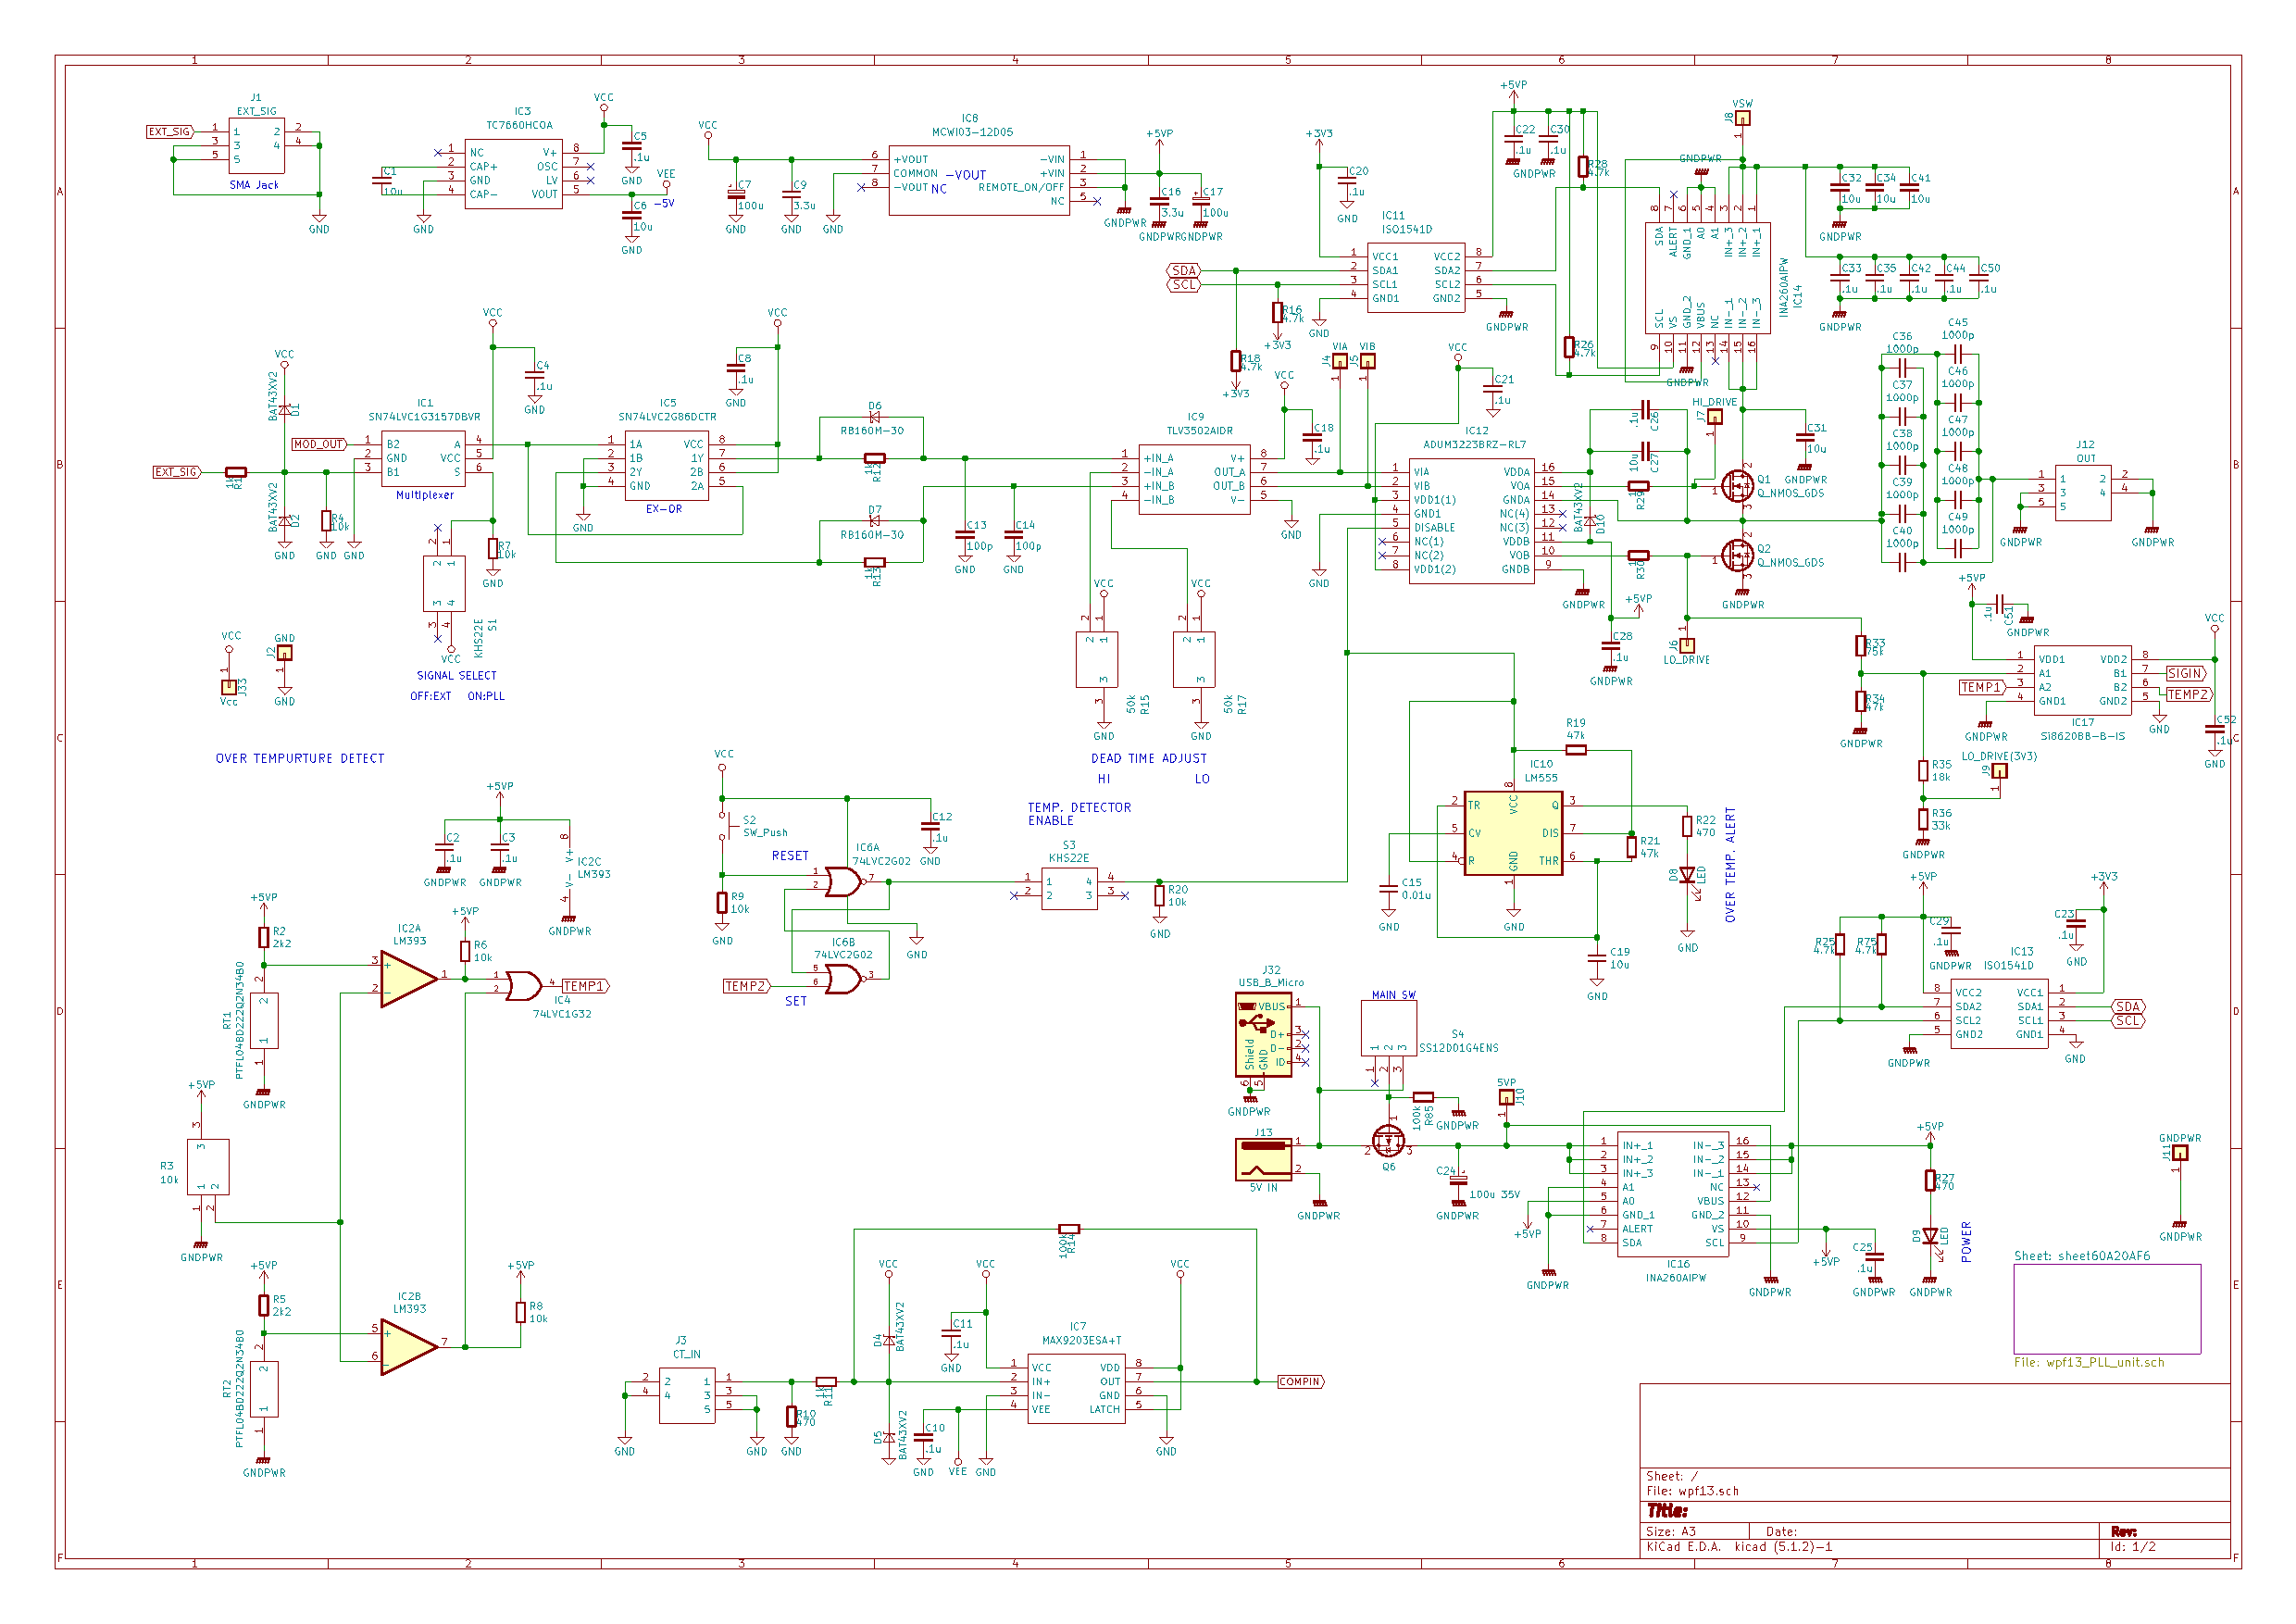
\includegraphics[width=220mm]{figures/wpf13_circuit1.pdf}
  \caption{送信側回路図(1/2)}

  \end{center}
\end{figure}
\end{landscape}


\begin{landscape}
\begin{figure}[p]
\begin{center}

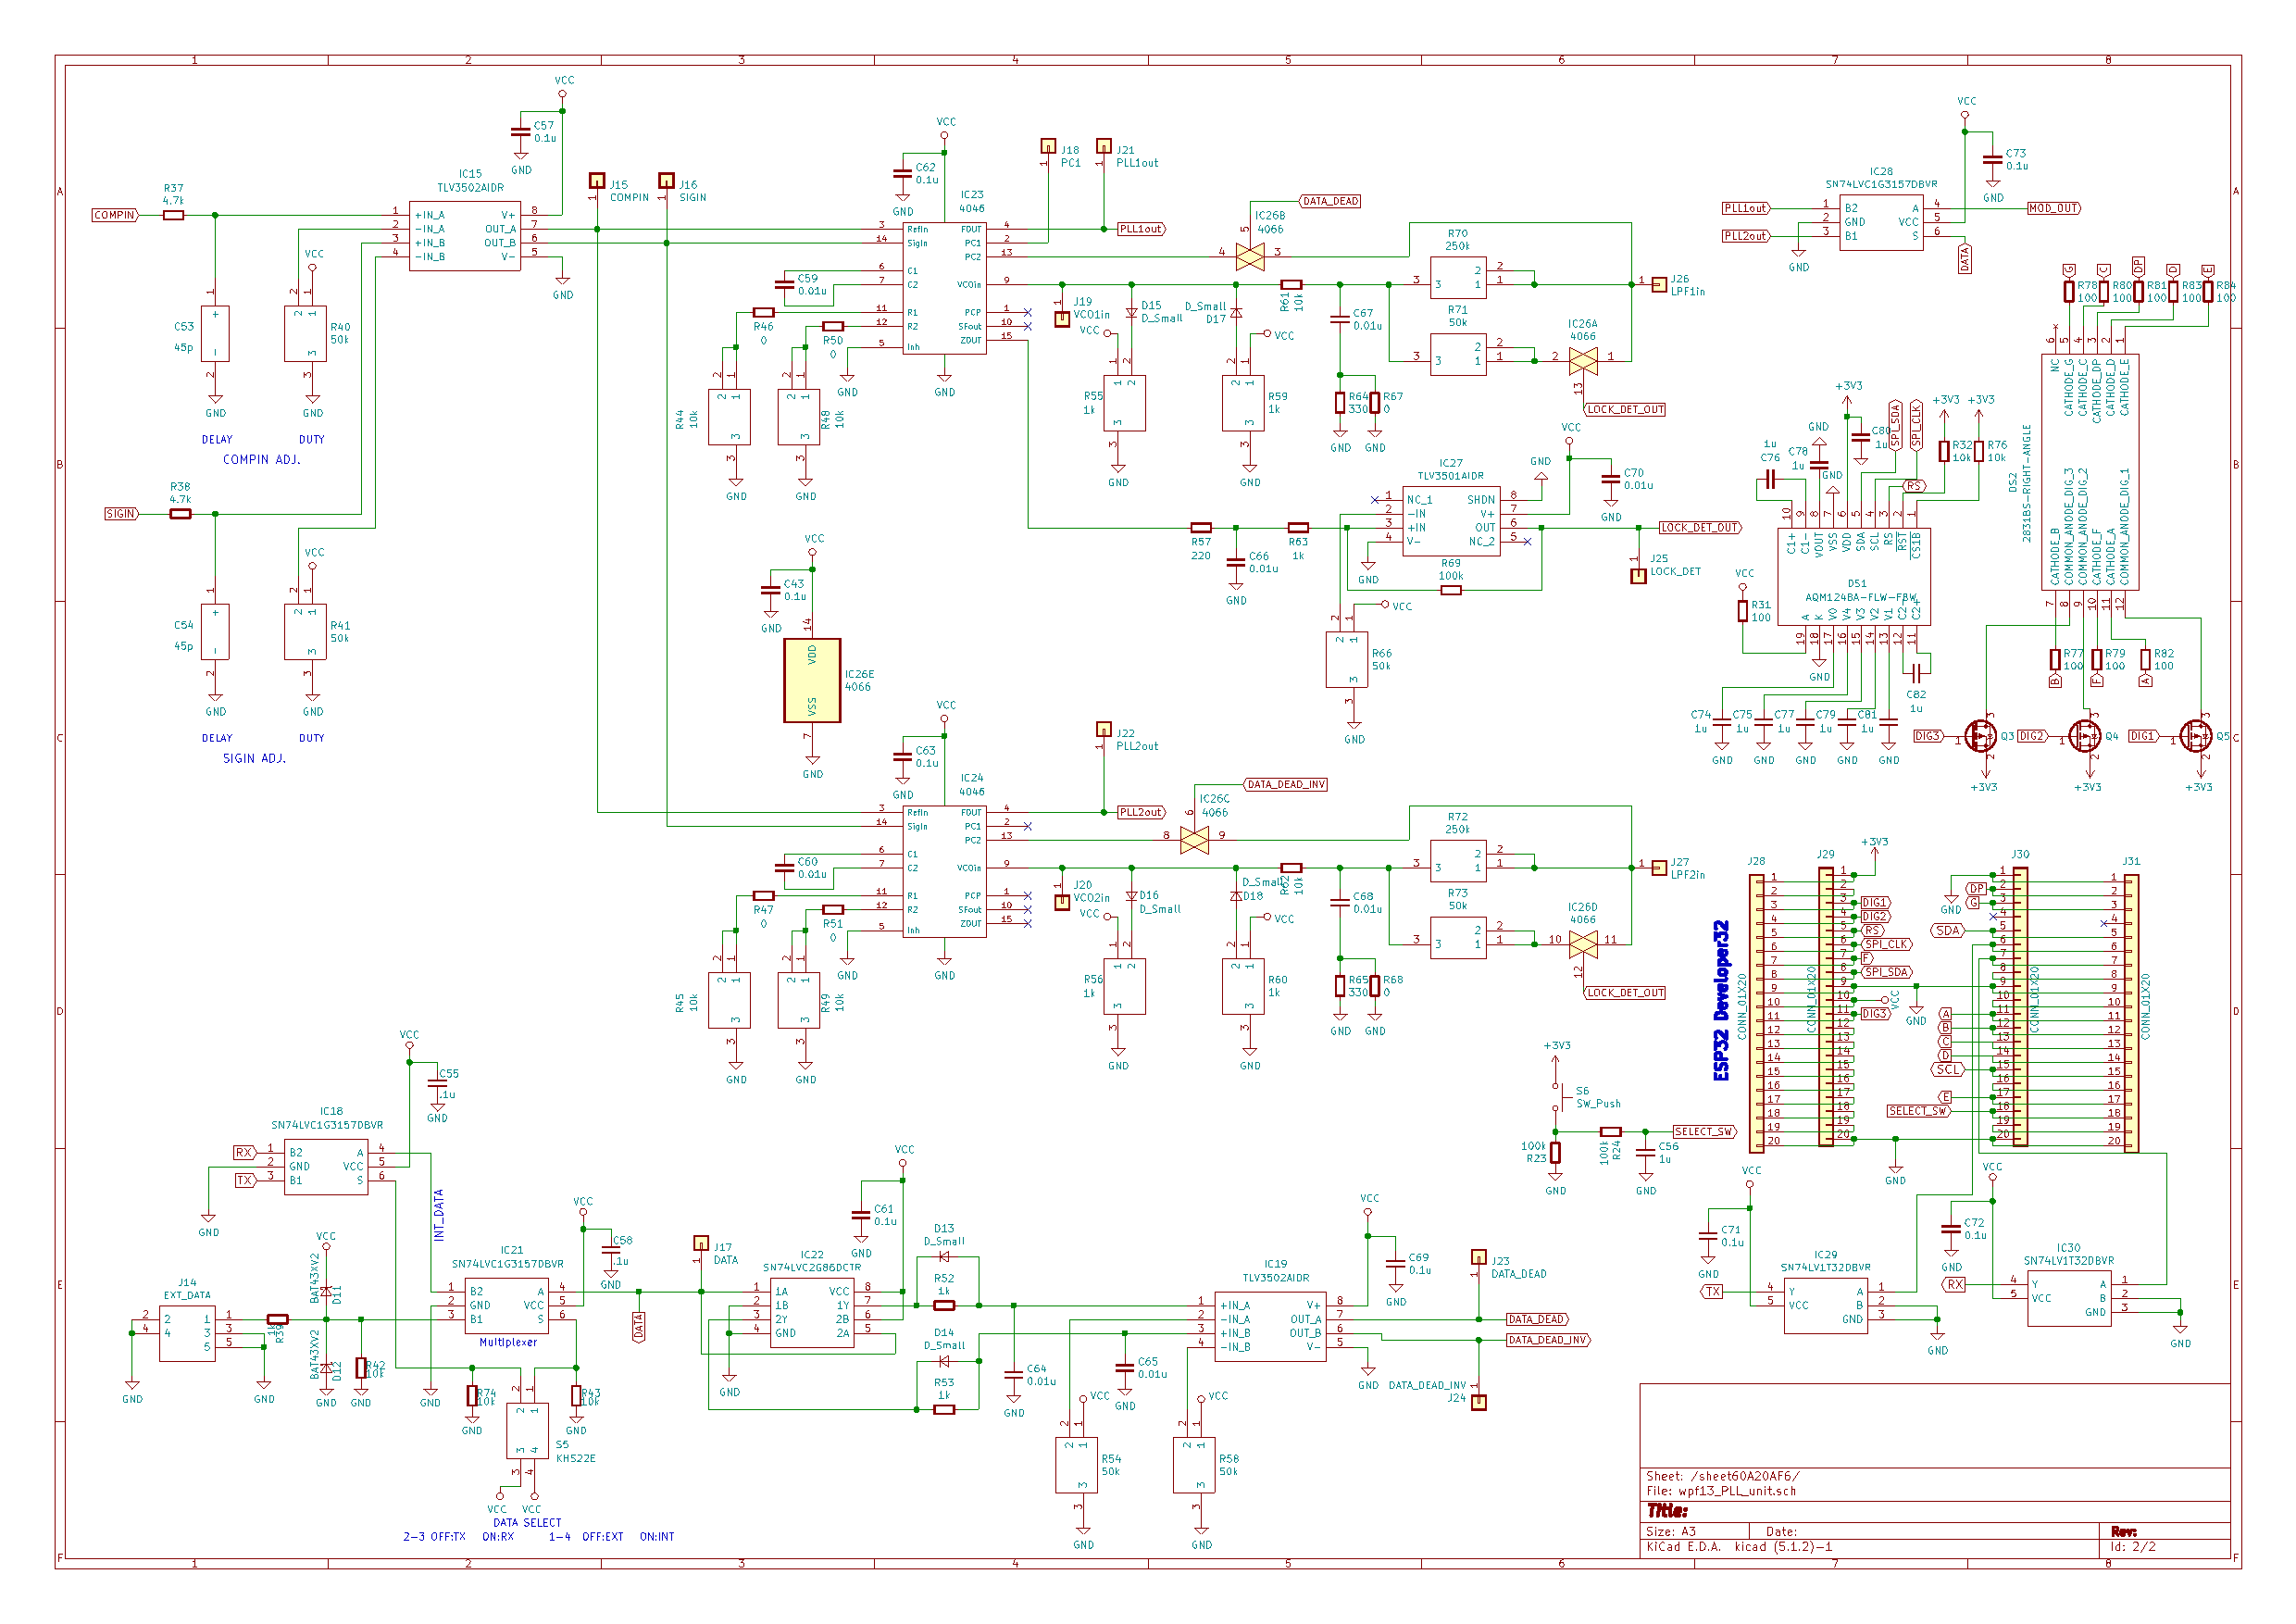
\includegraphics[width=220mm]{figures/wpf13_circuit2.pdf}
  \caption{送信側回路図(2/2)}

  \end{center}
\end{figure}
\end{landscape}


\begin{landscape}
\begin{figure}[p]
\begin{center}

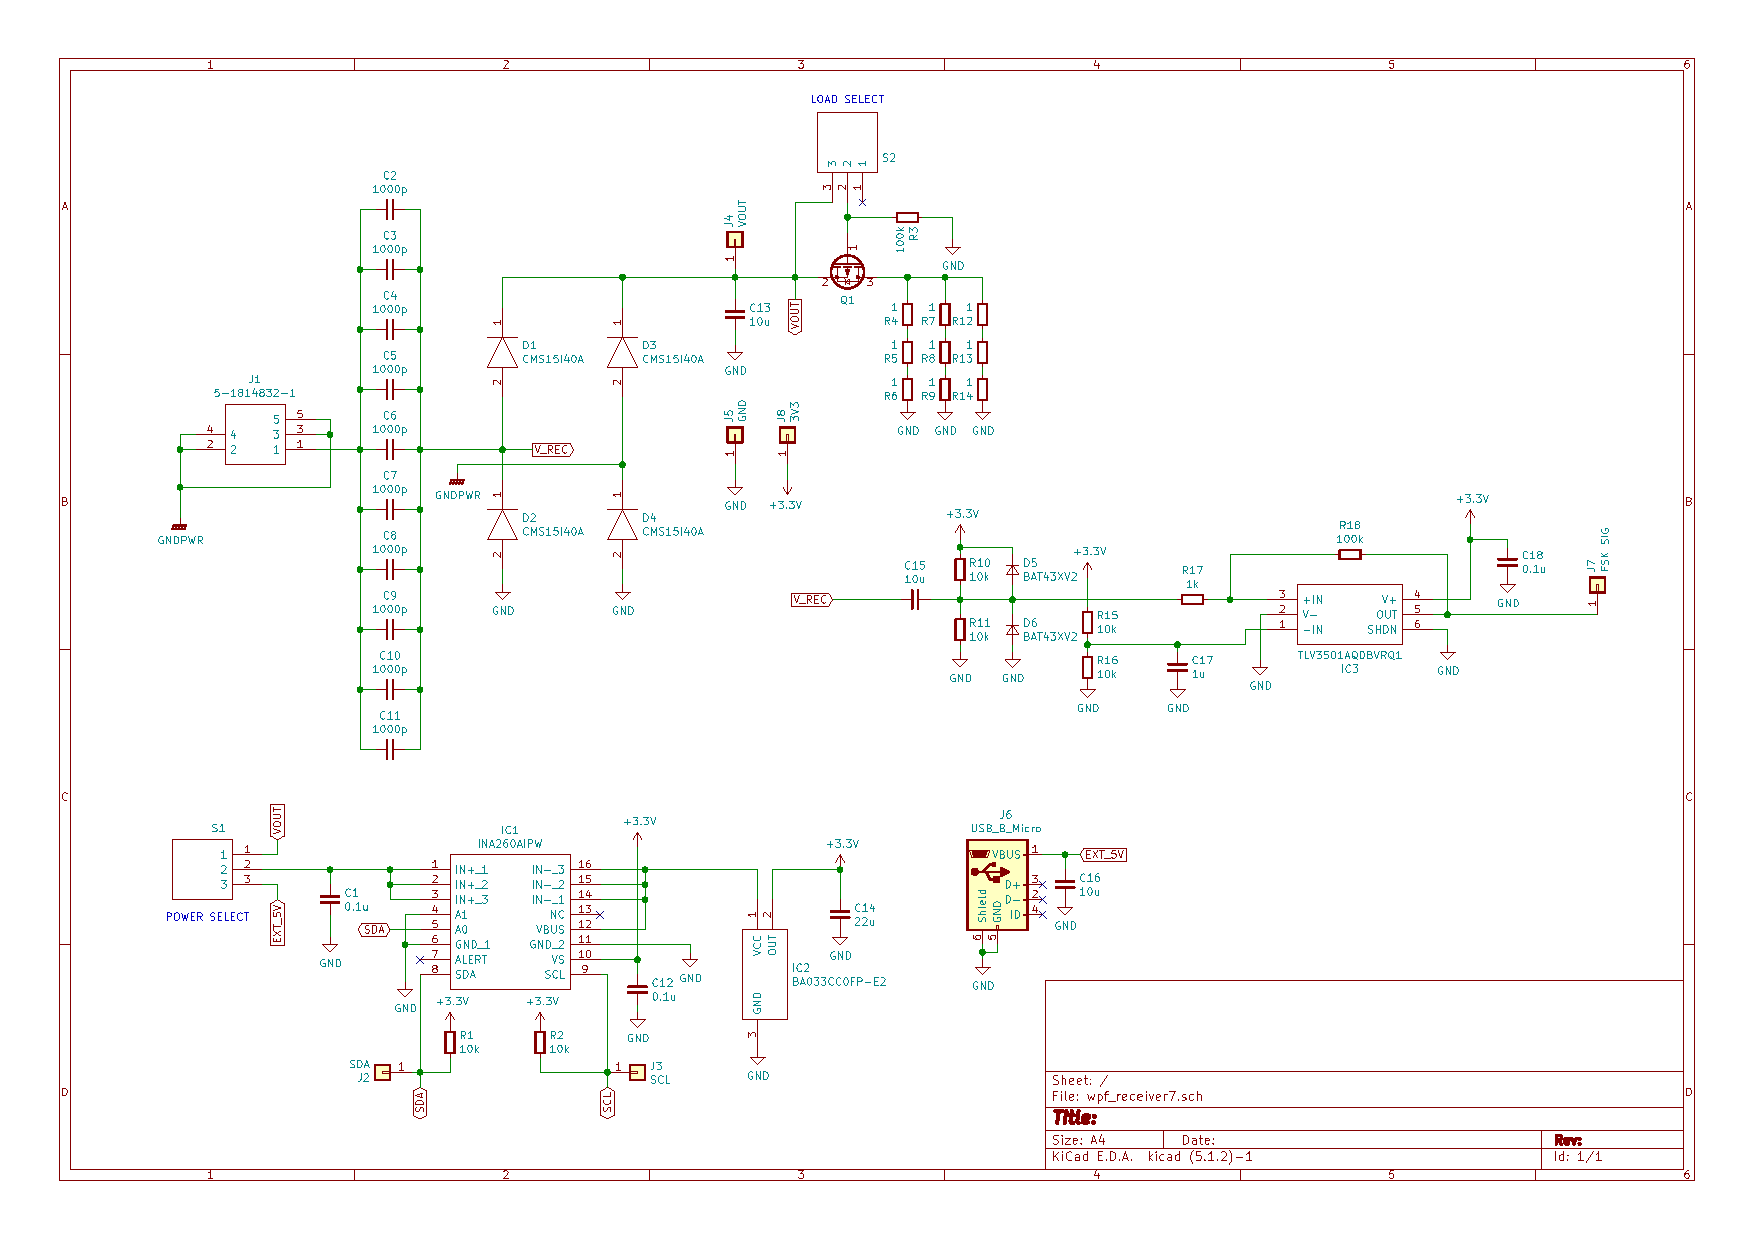
\includegraphics[width=220mm]{figures/wpf_receiver7_circuit.pdf}
  \caption{受信側回路図}

  \end{center}
\end{figure}
\end{landscape}


\begin{figure}[p]

	\begin{center}
    \subfloat[表面]{
    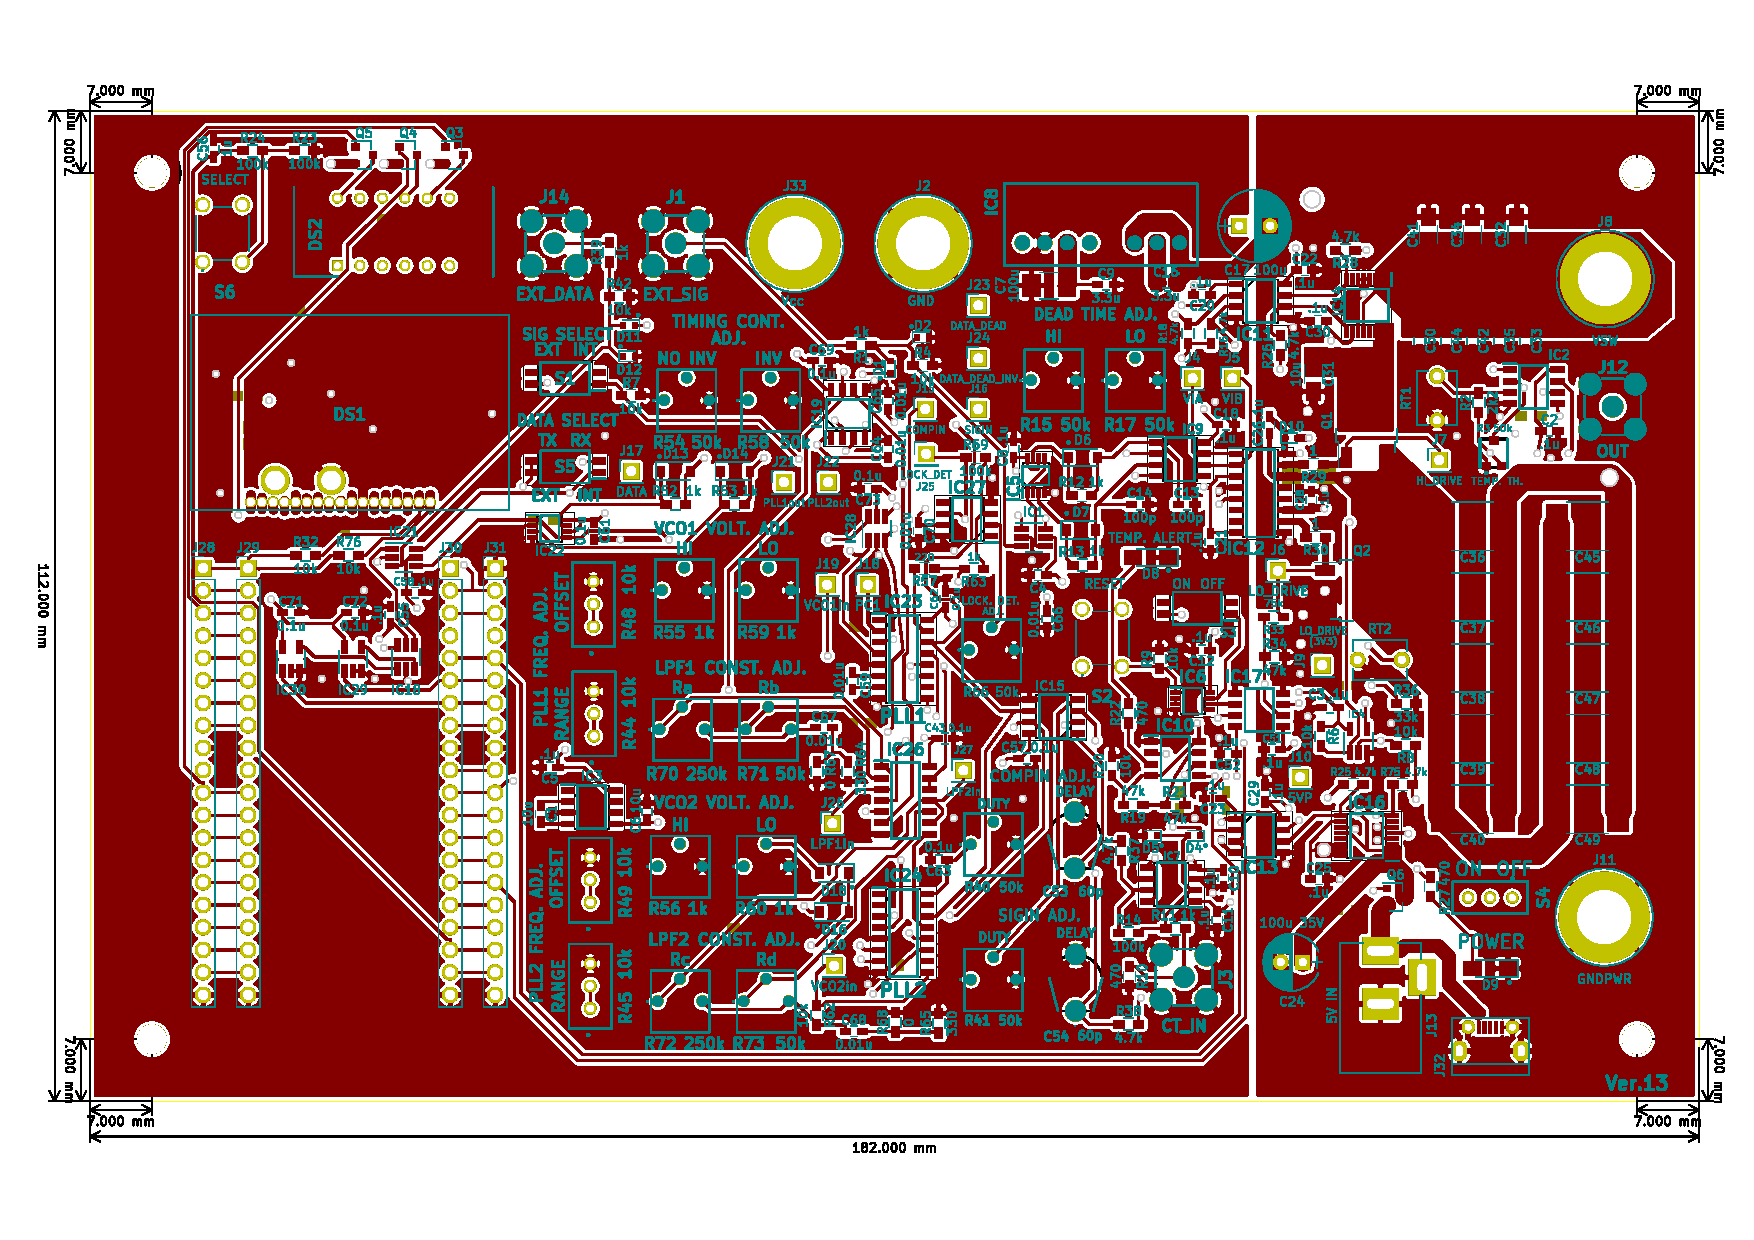
\includegraphics[width=150mm]{figures/wpf13_board_002.pdf}
    }
    \\ 
    \subfloat[内層1面]{
    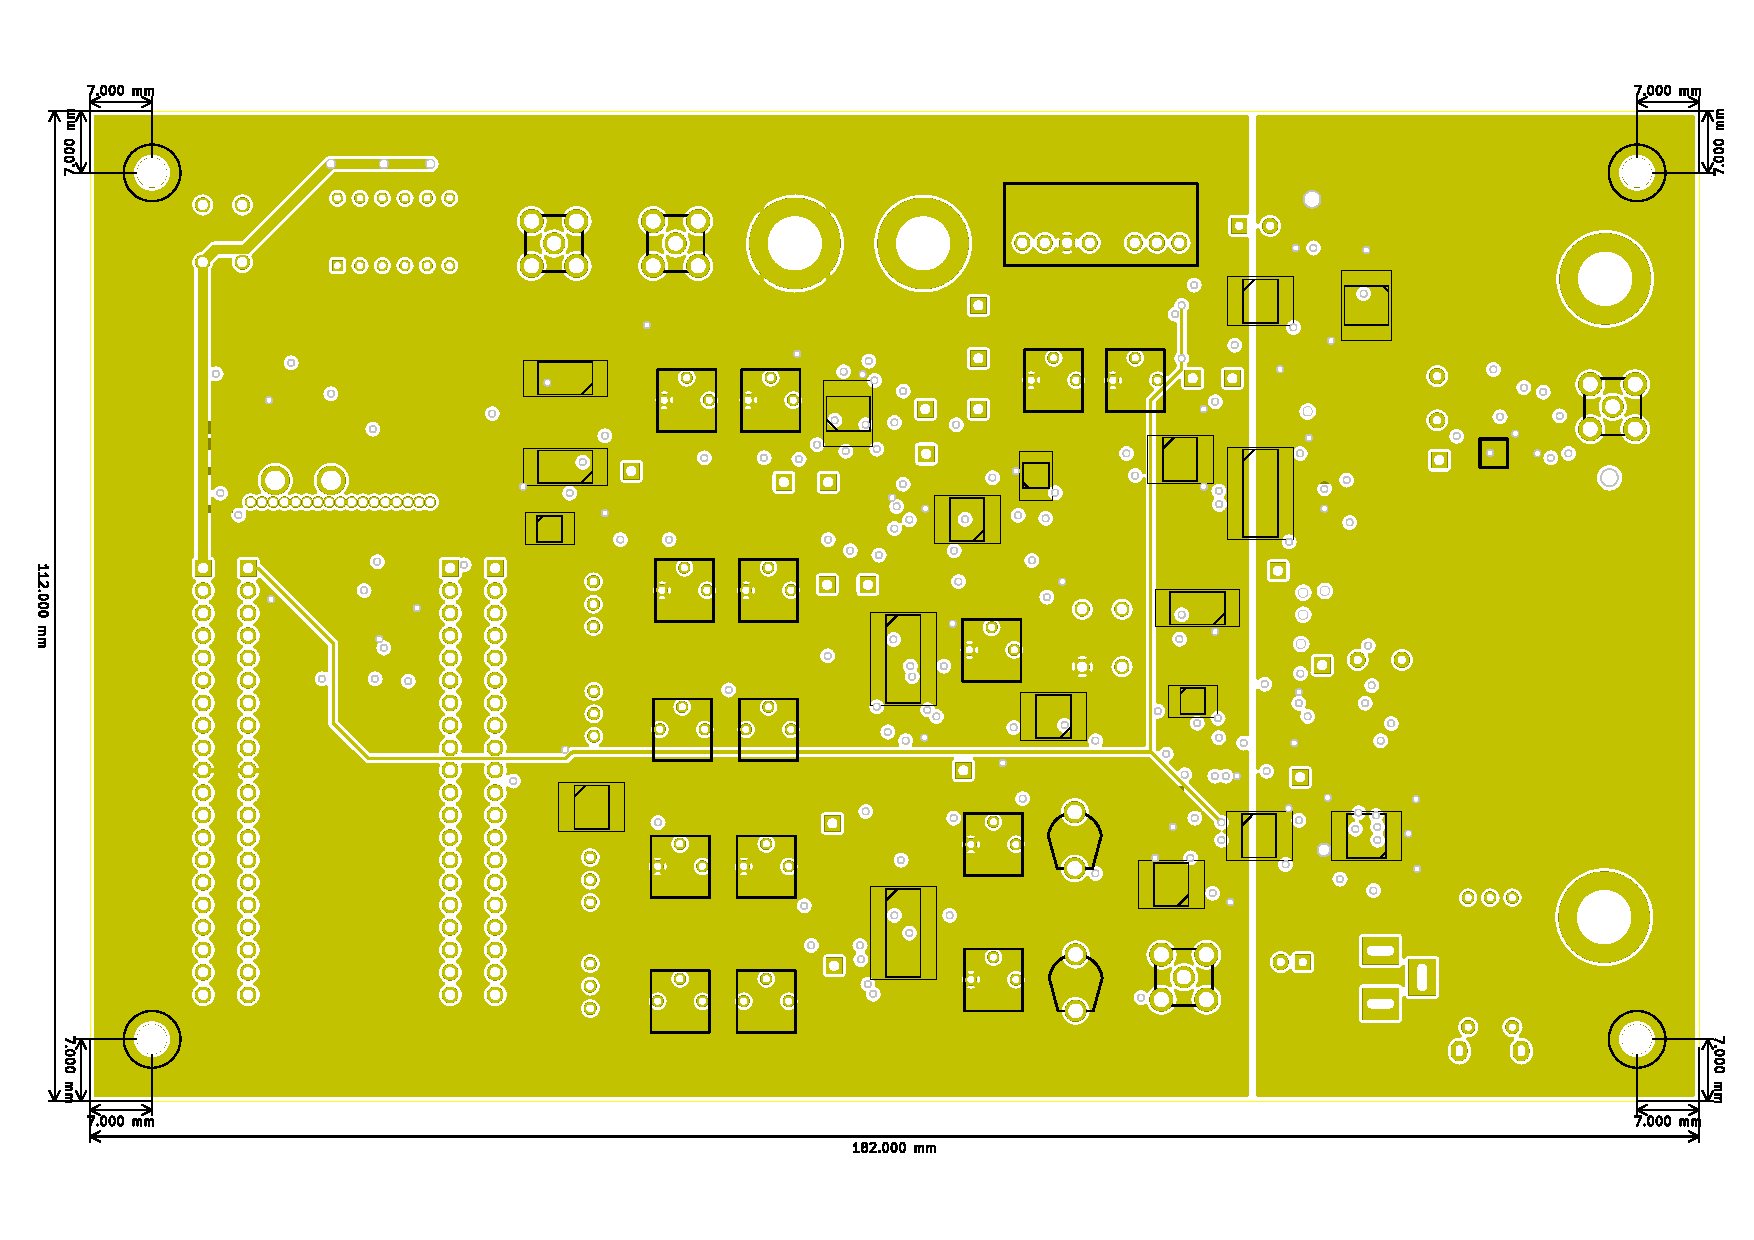
\includegraphics[width=150mm]{figures/wpf13_board_003.pdf}
    }
    \\ 
  \end{center}
\end{figure}

\begin{figure}[p]
	\begin{center}
    
    \setcounter{subfigure}{2}
    
    \subfloat[内層2面]{
    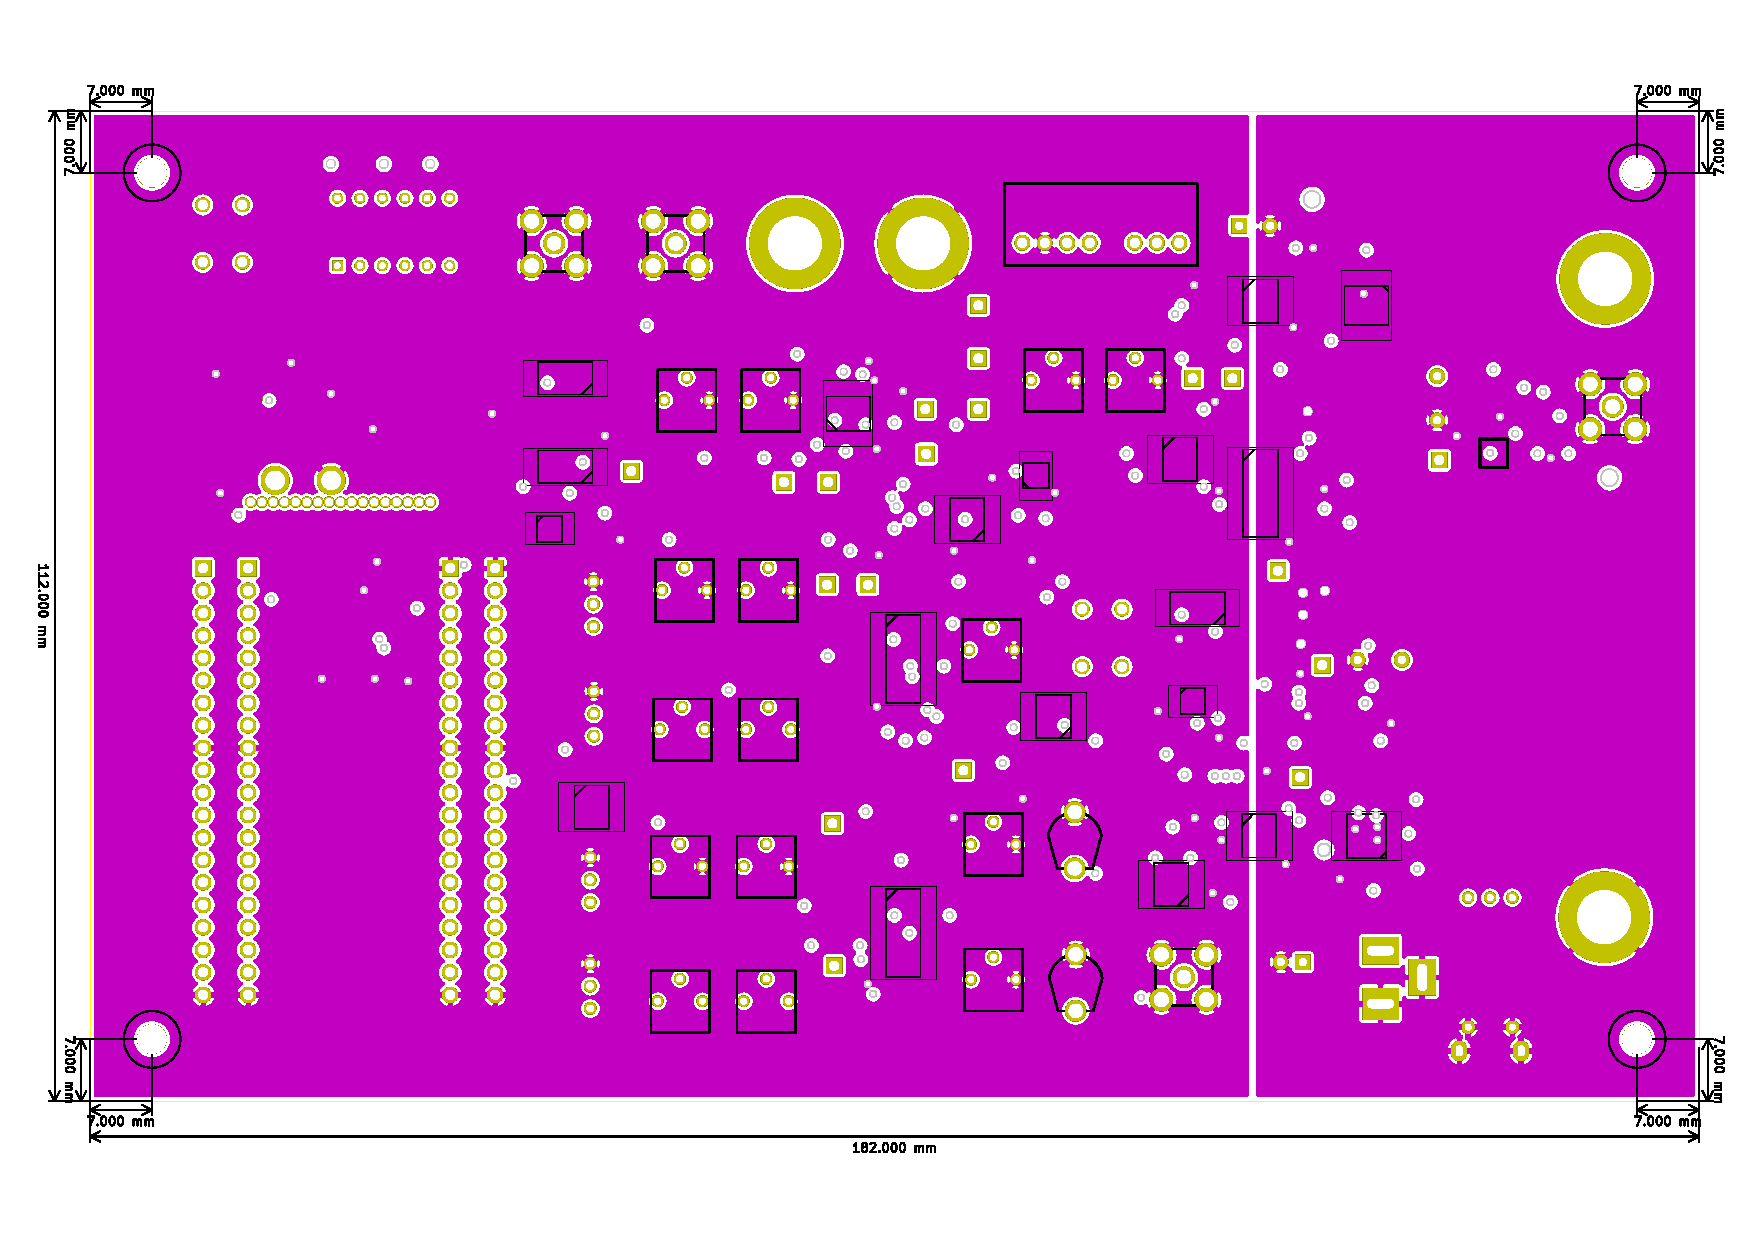
\includegraphics[width=150mm]{figures/wpf13_board_004.pdf}
    }
    \\ 
   
    \subfloat[裏面]{
    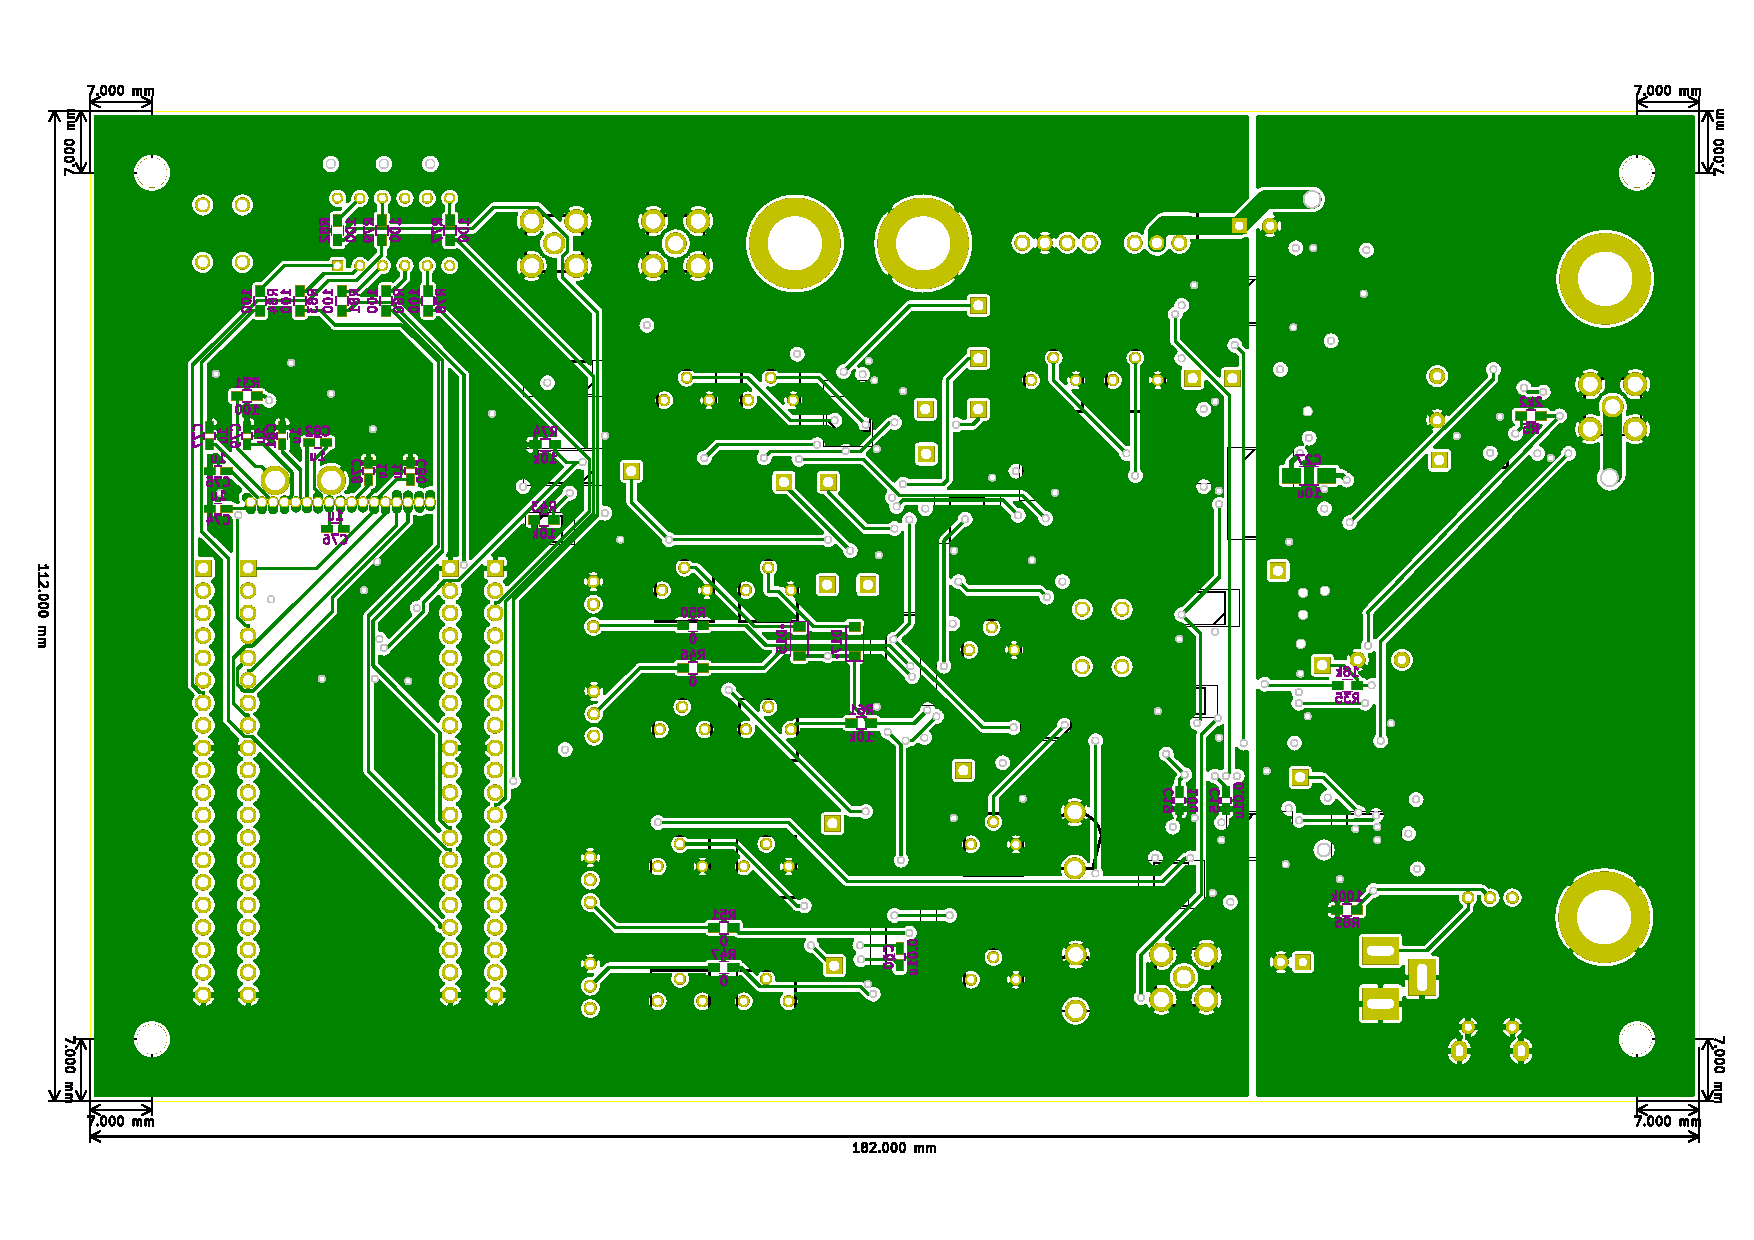
\includegraphics[width=150mm]{figures/wpf13_board_005.pdf}
    }

  \caption{送信側PCBレイアウト図}

    \end{center}
\end{figure}
  
  \begin{figure}[p]

	\begin{center}
    \subfloat[表面]{
    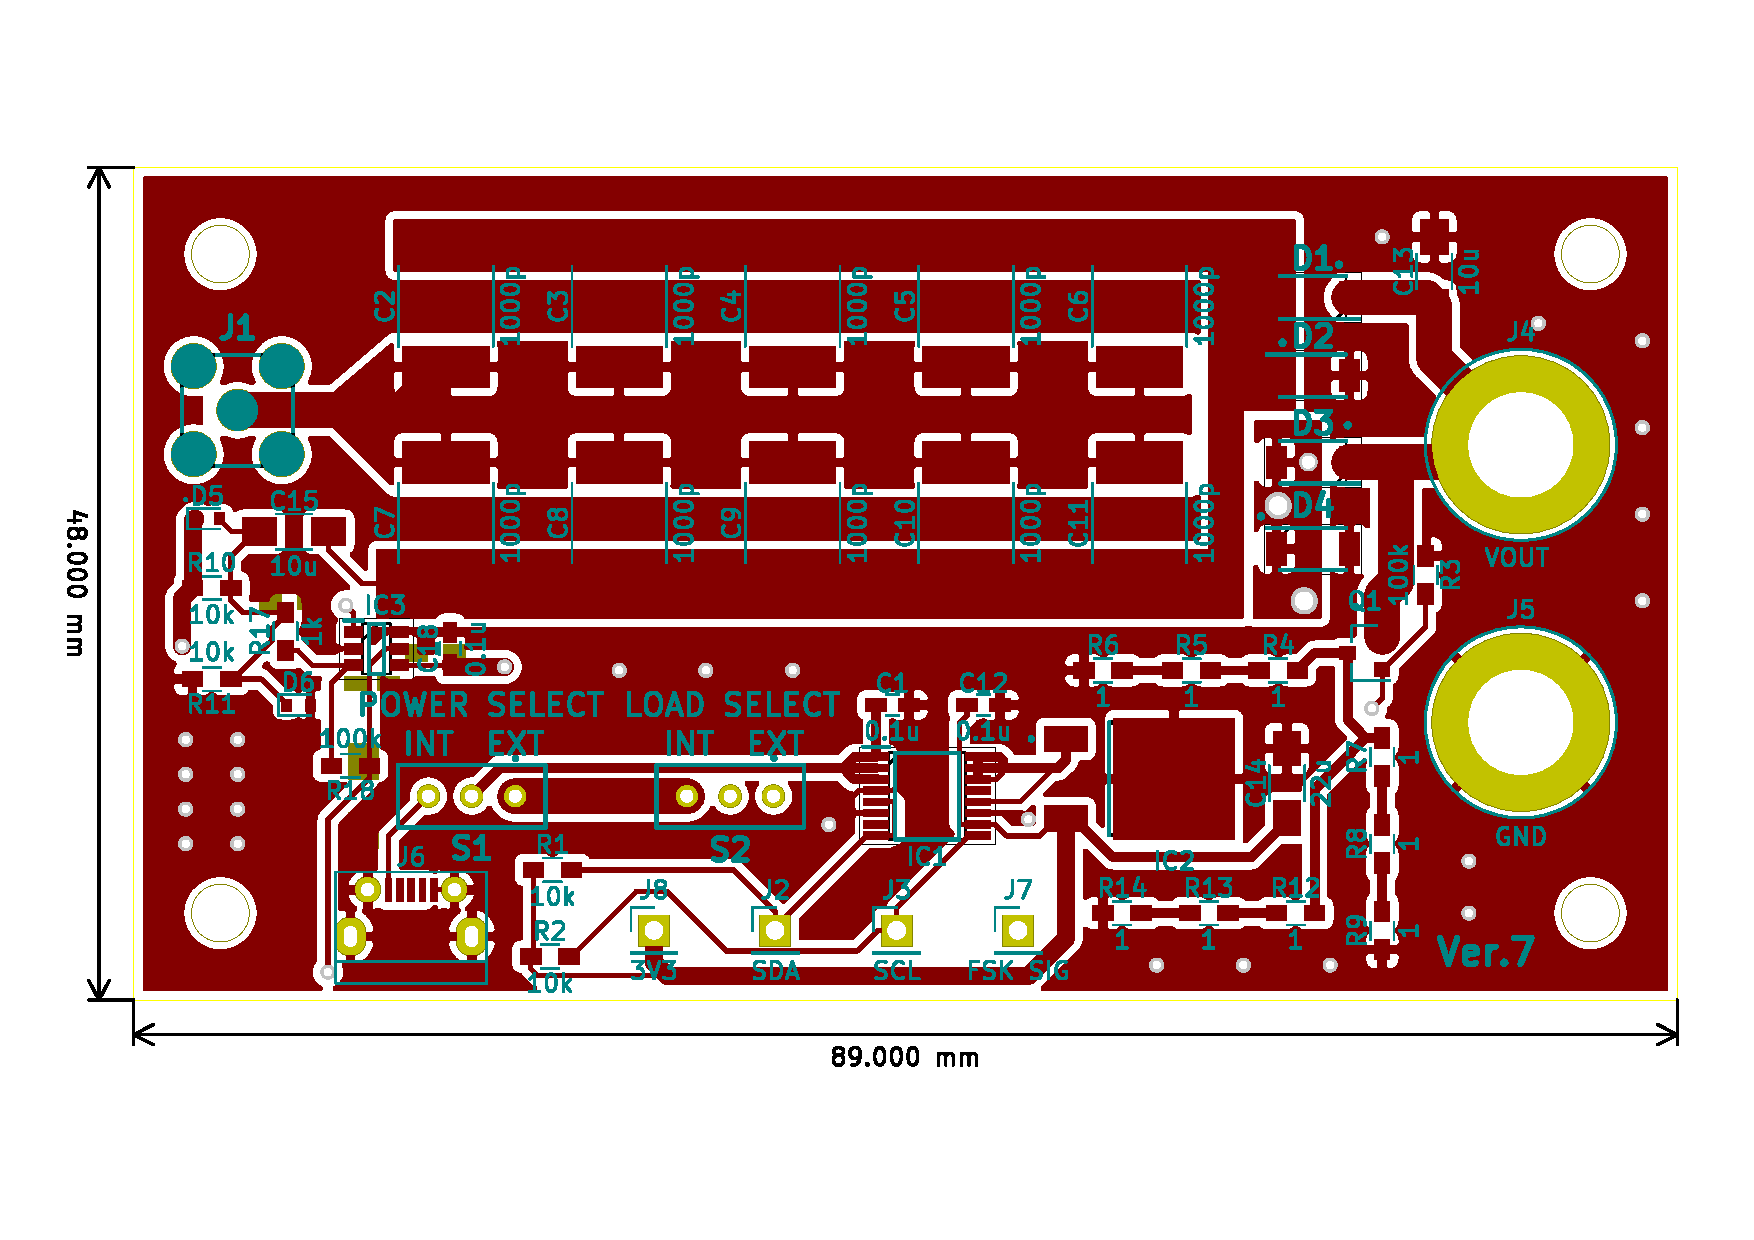
\includegraphics[width=150mm]{figures/wpf_receiver7_board_002.pdf}
    }
    \\ 
    \vspace{5mm}
    \subfloat[裏面]{
    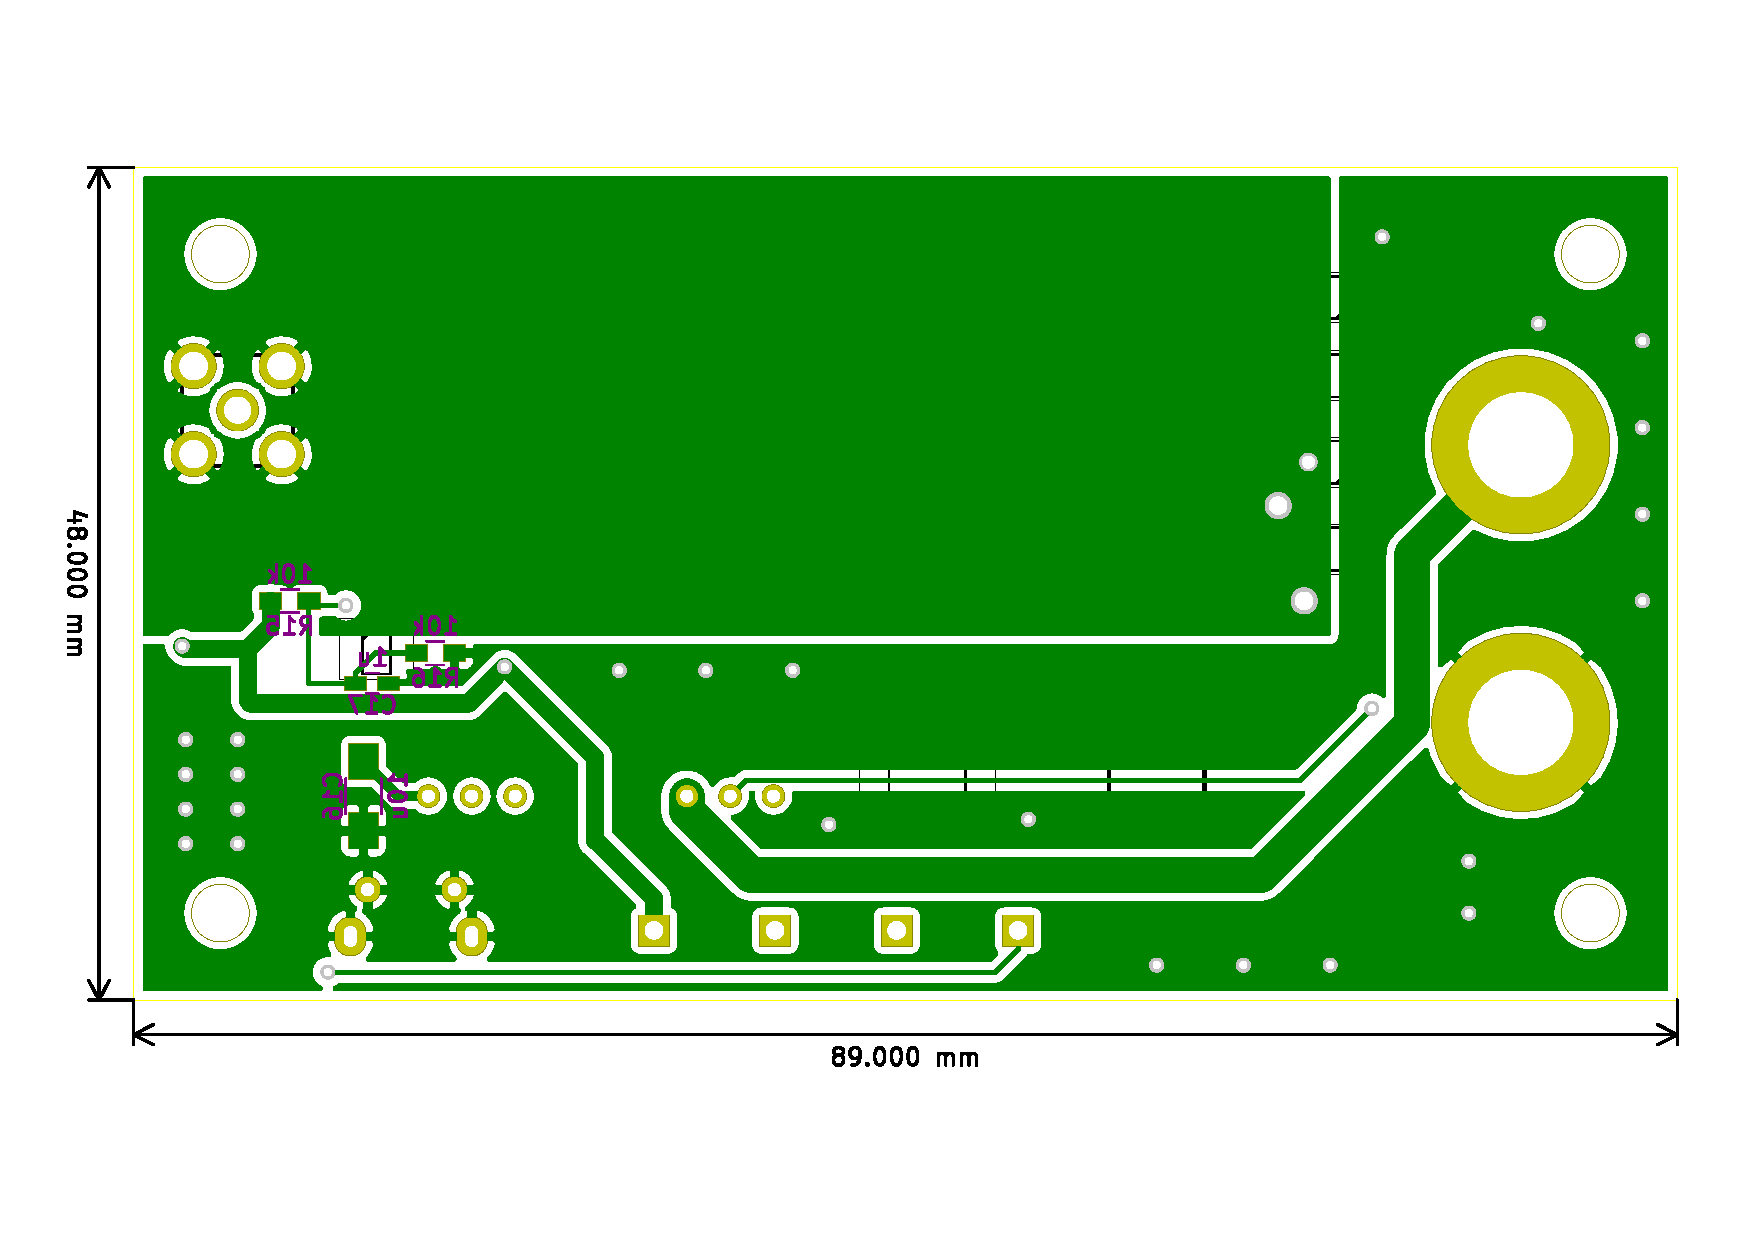
\includegraphics[width=150mm]{figures/wpf_receiver7_board_003.pdf}
    }
    \\ 
    \caption{受信側PCBレイアウト図}
  \end{center}
\end{figure}

\chapter{FSK復調器のVerilog-HDLソースコード}
FPGAを用いたFSK復調器のVerilog-HDLソースコードならびに論理シミュレーション用テストベンチを以下に示す.

\begin{lstlisting}[caption=FSK復調器]

module counter7_for_thesis(
    input clk,
    input serial_datain, 
    input sw0,
    input sw1,
    input sw2,
    input sw3,
    input btn0,
    input extfsksig, //b10
    
    output serial_dataout,
    output led0,
    output b1,
    output b2,
    output b3,
    output b4,
    output b7,
    output b8,
    output b9
        );  


parameter low_freq=598; /*kHzで指定*/  
parameter high_freq=979;
parameter integer cnt_fspace=(1/(low_freq*2*0.000008));
parameter integer cnt_fmark=(1/(high_freq*2*0.000008));  
parameter integer threshold=167;

reg [19:0] cntdata=20'd0;
reg [31:0] cntfspace=32'd0;
reg [31:0] cntfmark=32'd0;
reg [31:0] demodcnt_1p=32'd0;
reg [31:0] demodcnt_2p=32'd0;
reg [31:0] demodcnt_p=32'd0;
reg [31:0] difference_p=32'd0;
reg [31:0] bps=32'd0;
reg [31:0] rstpls_p=32'b0;
reg [63:0] resetcounter=64'd0; 

reg fmark=1'b0; /* high freq*/
reg fspace=1'b0; /*low freq*/
reg fsksig=1'b0;
reg fdata=1'b0;
reg datachange=1'b0;
reg demodout=1'b0;
reg cntrst_p=1'b0;    
reg resetflag=1'b0;
reg sigselect=1'b0;
reg recoverflag=1'b0;

initial @(negedge demodout) recoverflag<=1'b1;

always @(posedge clk)begin


/* set rate of pseudo data */
/////////////////////////////////////////////////////
       
         if(sw3==0 & sw2==0 & sw1==0& sw0==0) bps<='d300;
    else if(sw3==0 & sw2==0 & sw1==0& sw0==1) bps<='d600;
    else if(sw3==0 & sw2==0 & sw1==1& sw0==0) bps<='d1200;
    else if(sw3==0 & sw2==0 & sw1==1& sw0==1) bps<='d2400;
    else if(sw3==0 & sw2==1 & sw1==0& sw0==0) bps<='d4800;
    else if(sw3==0 & sw2==1 & sw1==0& sw0==1) bps<='d9600;
    else if(sw3==0 & sw2==1 & sw1==1& sw0==0) bps<='d14400;
    else if(sw3==0 & sw2==1 & sw1==1& sw0==1) bps<='d19200;
    else if(sw3==1 & sw2==0 & sw1==0& sw0==0) bps<='d38400;
    else if(sw3==1 & sw2==0 & sw1==0& sw0==1) bps<='d57600;
    else if(sw3==1 & sw2==0 & sw1==1& sw0==0) bps<='d115200;
    else if(sw3==1 & sw2==0 & sw1==1& sw0==1) bps<='d230400;
    else if(sw3==1 & sw2==1 & sw1==0& sw0==0) bps<='d460800;
    else if(sw3==1 & sw2==1 & sw1==0& sw0==1) bps<='d921600;
    else bps<='d115200;
    
/////////////////////////////////////////////////////


/*genarate pseudo FSK signal*/
/////////////////////////////////////////////////////
    if(cntfspace == cnt_fspace) begin
        cntfspace<=32'd0; // reset cnt //
        fspace<=~fspace;
 end
        
else begin
    cntfspace<=cntfspace+32'd1;
 end
 
////////////////////////////////////////////
 
     if(cntfmark == cnt_fmark) begin
        cntfmark<=32'd0; // reset cnt //
        fmark<=~fmark;
 end
        
else begin
    cntfmark<=cntfmark+32'd1;
 end
 
////////////////////////////////////////////

      if(cntdata == 'd125000000/bps) begin
        cntdata<=20'd0; // reset cnt //
       fdata<=~fdata;
 end
        
else begin
    cntdata<=cntdata+20'd1;
 end
 
///////////////////////////////////////////////////// 
  
  
/*choose internal(pseudo) or external FSK signal*/
/////////////////////////////////////////////////////
 
 if(btn0==1) sigselect<=~sigselect;
 
 if(sigselect==0) begin
 
    if(fdata==0)   begin
    fsksig<=fspace;
    end
     else begin
    fsksig<=fmark;
    end
 end
 
 if(sigselect==1) fsksig<=extfsksig;
 
/////////////////////////////////////////////////////


/*generate counter-reset pulse*/
/////////////////////////////////////////////////////

if(fsksig==1'b1) begin  
    rstpls_p<=rstpls_p+1'b1;
        if(rstpls_p<1'b1) cntrst_p<=1'b1;
        else if (rstpls_p==1'b1) begin
        rstpls_p<=1'b1;
        cntrst_p<=1'b0;
        end

end

if(fsksig==1'b0) rstpls_p<=1'b0;
/////////////////////////////////////////////////////


/*set counter*/
/////////////////////////////////////////////////////
 
  if(fsksig==1'b0 && cntrst_p==1'b0)      demodcnt_2p<=demodcnt_2p+32'd1;
 else if (fsksig==1'b1 && cntrst_p==1'b0)    demodcnt_1p<=demodcnt_1p+32'd1;
 else begin
    demodcnt_1p<=32'd0;
    demodcnt_2p<=32'd0;
 end
 
 demodcnt_p<=demodcnt_1p+demodcnt_2p;
 
///////////////////////////////////////////////////// 
 
 
/*set normally HIGH*/
/////////////////////////////////////////////////////
if(cntrst_p==1'b1) begin
    if(demodcnt_1p>demodcnt_2p) difference_p<=demodcnt_1p-demodcnt_2p;
    if(demodcnt_2p>demodcnt_1p) difference_p<=demodcnt_2p-demodcnt_1p;
    if(demodcnt_1p==demodcnt_2p) difference_p<=0;
end

if(difference_p>'d10) datachange<=1'b1;
else datachange<=1'b0;

////////////////////////////////////////////

if(datachange==0)begin                      // set normally high
    resetcounter<=resetcounter+32'd1;
    
    if(resetcounter>'d125000000) resetflag<=1'b1; else resetflag<=1'b0;
end

if(datachange==1) resetcounter<=32'd0;
    
/////////////////////////////////////////////////////


/* data detection */
/////////////////////////////////////////////////////

if(cntrst_p==1'b1) begin
        if(demodcnt_p>threshold) demodout<=1'b0;
        if(demodcnt_p<threshold) demodout<=1'b1;
    end 
    
   else demodout<=demodout;
   
///////////////////////////////////////////////////// 
 end
 
assign b1=fdata;
assign b2=fmark;
assign b3=fspace;
assign b4=fsksig;
assign b7=demodout;
assign b8=cntrst_p;
assign b9=datachange;
assign led0=sigselect;
assign serial_dataout=demodout;
endmodule

\end{lstlisting}


\begin{lstlisting}[caption=テストベンチ]

`timescale 1ns / 1ps

module counter7_tb;
    
    reg clk;
    reg rnd;
    
    wire sw0=0;
    wire sw1=0;
    wire sw2=0;
    wire sw3=1;
    wire btn0=0;
    wire extfsksig=0;
           
    wire serial_dataout;
    wire led0;
    wire b1;
    wire b2; 
    wire b3; 
    wire b4;
    wire b7;
    wire b8;
    wire b9;
   
    initial clk<=0;
  
    always  #4 clk=~clk;
    
    counter7_for_thesis uut(
    .clk(clk), 
    .serial_datain(rnd),
    
    .sw0(sw0),
    .sw1(sw1),
    .sw2(sw2),
    .sw3(sw3),
    .btn0(btn0),
    .extfsksig(extfsksig),
    
    .serial_dataout(serial_dataout),
    .led0(led0),
    .b1(b1), 
    .b2(b2), 
    .b3(b3),
    .b4(b4),
    .b7(b7),
    .b8(b8),
    .b9(b9));
endmodule
\end{lstlisting}


\end{document}
